% !TEX encoding = UTF-8
% !TEX program = xelatex
\documentclass[10pt,b5paper, openany]{book} %openany: 新章节不强制从奇数页开始

% 调整页边距
\usepackage{geometry}
\geometry{right=1.6cm,left=1.6cm,top=2.3cm,bottom=2cm}

% 调整行距
\usepackage{setspace}

% 设置中文字体
\usepackage[UTF8, fontset=none]{ctex}
\usepackage{fontspec}
\xeCJKDeclareCharClass{CJK}{%  %使Unicode带圈字符正确显示
  "24EA,           %
  "2460->"2473,    %
  "3251->"32BF,    %
  "24FF,           %
  "2776->"277F,    %
  "24EB->"24F4     %
}
\setCJKmainfont[BoldFont = 思源黑体, ItalicFont = 华文楷体]{思源宋体}
\setmonofont{等距更纱黑体 SC}
\setCJKmonofont{等距更纱黑体 SC}

% ams大礼包
\usepackage{amsmath}
\DeclareMathOperator{\Tr}{Tr} % 自定义 trace
\DeclareMathOperator{\tr}{tr}
\usepackage{amssymb}
\usepackage{amsfonts}

% slashed letters
\usepackage{cancel}

% 删除线 波浪线 斜删除线 双下划线
\usepackage{ulem}
% \sout{文字} %删除线
% \uwave{文字} %波浪线
% \xout{文字} %斜删除线
% \uuline{文字}  %双下划线

% 输入数组矩阵
\usepackage{array}

% 输入正体希腊字母
\usepackage{upgreek}

% 调整参考文献引用格式
\usepackage{cite}

% 超链接
\usepackage{hyperref}
\hypersetup{
  colorlinks=true,
  linkcolor=red!80!black,
  urlcolor=Cyan!60!black,
}

% 文字颜色
\usepackage[dvipsnames]{xcolor}

% 插入图片等
\usepackage{graphicx}
\graphicspath{
  {./image/}
}

% 浮动体标题的格式
\usepackage{caption}

% 给符号加粗用
\usepackage{bm}

% 调整 pdf 大纲格式
\usepackage{hyperref}
\hypersetup{
    bookmarksnumbered=true, 
    % bookmarksdepth=section,
}

% 调整页眉章节标题样式
\usepackage{fancyhdr}
\fancypagestyle{general}{
  \fancyhf{} % 清空当前页眉和页脚的设置

  % 设置页眉
  \fancyhead[LE]{{\bfseries \thepage}\quad\quad\nouppercase{\leftmark}}
  \fancyhead[RE]{}
  \fancyhead[RO]{\nouppercase{\rightmark}\quad\quad{\bfseries \thepage}}
  \fancyhead[LO]{}
}

% 漂亮的文本框
\usepackage{tcolorbox}
\tcbuselibrary{skins, breakable}

% 命令
% 长横线
\newcommand{\HRule}{\rule{\linewidth}{0.5mm}} 

% 文本框
\newtcolorbox{mybox}[2][]{
  center,
  width=0.98\linewidth,
  breakable,
  boxrule=1pt,
  colbacktitle=black!5!white,
  colback=white,
  coltitle=black,
  title={#2},
  fonttitle=\itshape,
  #1}

% 着重号
\usepackage{xeCJKfntef}
\xeCJKsetup{underdot/symbol={\normalfont^^b7}}
\newcommand{\cemph}[1]{\CJKunderdot{#1}}
% \newcommand{\cemph}[1]{#1}

% 无标号 chapter (改变页眉页脚格式)
\newcommand{\nonumchap}[1]{
  \fancypagestyle{nonumchap}{
    \fancyhead[LE]{{\bfseries \thepage}\quad\quad{#1}}
  }
  \pagestyle{nonumchap}
  \phantomsection % 加这个命令后, 目录中的超链接才指向正确的页码
  \chapter*{#1} %开始一段不带编号的章
  \addcontentsline{toc}{chapter}{#1} %使目录中以章级别显示
}

% 无标号 chapter (保持页眉页脚格式)
\newcommand{\nonumchapkphdr}[1]{
  \phantomsection % 加这个命令后, 目录中的超链接才指向正确的页码
  \chapter*{#1} %开始一段不带编号的章
  \addcontentsline{toc}{chapter}{#1} %使目录中以章级别显示
}

% 无标号 section (改变页眉页脚格式)
\newcommand{\nonumsec}[1]{
  \fancypagestyle{nonumsec}{
    \fancyhead[RO]{{#1}\quad\quad{\bfseries \thepage}}
  }
  \pagestyle{nonumsec}
  \phantomsection 
  \section*{#1} 
  \addcontentsline{toc}{section}{#1}
}

% 无标号 section (保持页眉页脚格式)
\newcommand{\nonumseckphdr}[1]{
  \phantomsection 
  \section*{#1} 
  \addcontentsline{toc}{section}{#1}
}

% 无标号 subsection
\newcommand{\nonumssec}[1]{
  \phantomsection 
  \subsection*{#1} 
  \addcontentsline{toc}{subsection}{#1}
}

\begin{document}
\pagestyle{fancy}

\begin{titlepage}
  \centering

  \HRule \\[0.7cm]

  {\bfseries \fontsize{35pt}{1pt}\selectfont \xeCJKsetup{CJKglue=\hskip 1.5pt}QFT笔记} \\[0.3cm]

  {\fontsize{14pt}{1pt}\selectfont based on the textbook by {\bfseries Peskin \& Schroeder}} \\[0.4cm]

  \HRule \\[0.6cm]

  {\Large tinikov} \\[0.2cm]

  {\small 创建于2021年10月29日} \\[-0.1cm]

  {\small 更新于\today} \\[0cm]

  \center{
    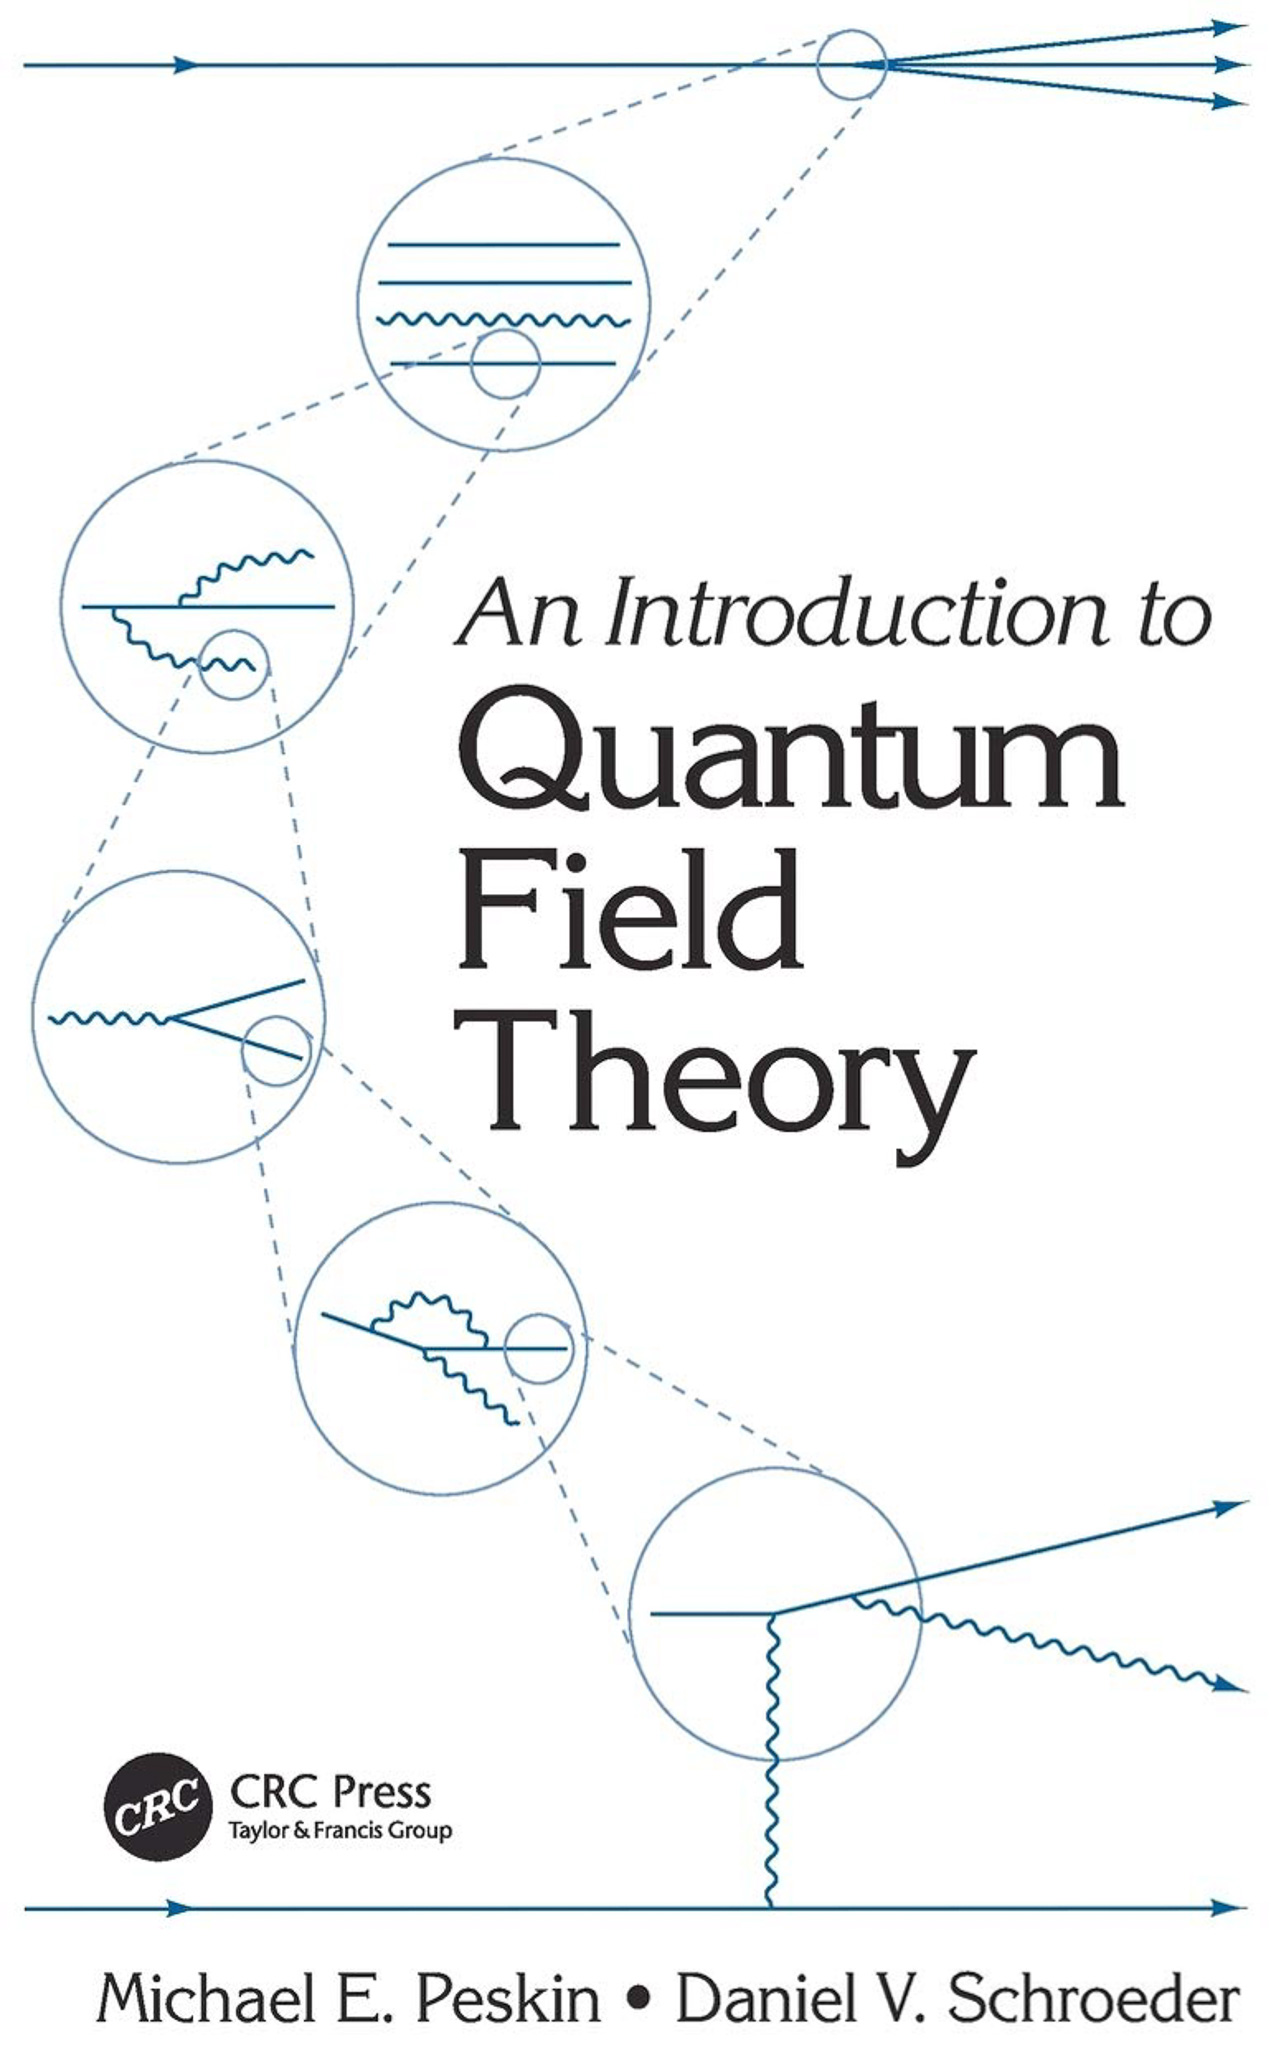
\includegraphics[width=0.6\textwidth]{peskin-front.jpg}
  }
\end{titlepage}

\pagenumbering{roman}
\setcounter{page}{1}
\nonumchap{前言}

\begin{spacing}{1.8}
  本书为基于\textit{An Introduction to Quantum Field Theory} - \textit{Peskin \& Schroeder}的量子场论笔记.

  \mbox{}

  本书主要对Peskin书中正文部分一些复杂(或不太复杂)的计算和难以理解(指我不理解)的段落作了注释, 同时根据研究生课程内容对部分较为简略的段落添加了补充说明, 希望对场论的初学者(比如说我)有一定的参考意义.
  由于解释说明较为困难, 故此笔记以中文呈现.
  \sout{若有闲暇, 可能翻译为英文. }

  \mbox{}

  本书参考了\href{http://gamebm.shoutwiki.com/wiki/Lecture_Notes_of_An_Introduction_to_Quantum_Field_Theory_by_M._Peskin_and_D._Schroeder}{这篇笔记} (谢谢你, 陌生人).
  如果学了一段时间场论以后感到一头雾水的话, 不妨参考Yuchen Wang (非常厉害的一个人!)的\href{https://zhuanlan.zhihu.com/p/391450897}{笔记}.

  特别感谢好友Starry的增补及校对.

  \mbox{}

  如发现任何错误或遗漏, 或希望与我讨论书中的内容, 欢迎通过\href{mailto:tinikov137@gmail.com}{邮件}联系.

  我的邮箱: \texttt{tinikov137@gmail.com}
\end{spacing}
\pagestyle{general}
\clearpage

\phantomsection
\addcontentsline{toc}{chapter}{目录}
{
  \hypersetup{linkcolor=black}
  \tableofcontents
}
\clearpage

\begin{spacing}{1.2}
  \pagenumbering{arabic}
  \setcounter{page}{1}
  \part{Feynman Diagrams and Quantum Electrodynamics}

  \pagestyle{general}
  \chapter{Invitation: Pair Production in \texorpdfstring{$e^+e^-$}\ \ Annihilation}

\nonumsec{Summary}
本章介绍了本书第一部分的主要目标:
\begin{enumerate}
  \item 计算$e^+e^-\rightarrow \mu^+\mu^-$这一过程的散射截面(这也是QED中最简单的过程)
  \item 看懂Feynman图并且能够用它计算一些简单的过程(因为没有涉及重整化, 基本只能计算tree level的图)
\end{enumerate}
\pagestyle{fancy}


  \pagestyle{general}
  \chapter{The Klein-Gordon Field}

\nonumsec{Summary}
\begin{itemize}
  \item 整章内容都是基础, 需要掌握所有公式的推导
  \item Peskin \& Schroeder对标量场进行量子化(从书中第20页开始)的方法很奇怪, 可直接参考笔记 \ref{subsubsec: KG_Field_expression} 一节中的方法——①\ 求得标量场运动方程的解; ②\ 利用等时对易关系(此时已经将场看作了算符)计算场展开式中系数(也是算符)的对易关系
  \item 正则量子化定义了单粒子态:
        \begin{equation*}
          |\mathbf{p}\rangle = \sqrt{2E_{\mathbf{p}}}a^{\dagger}_{\mathbf{p}}|0\rangle
        \end{equation*}
  \item Noether守恒荷($j^\mu$为Noether守恒流):
        \begin{equation*}
          Q \equiv \int j^0\ d^3x \quad (\int \text{in\ all\ space})
        \end{equation*}
  \item 能动量张量:
        \begin{equation*}
          T^{\mu}_{\phantom{\mu}\nu}\equiv \frac{\partial \mathcal{L}}{\partial (\partial_{\mu} \phi)} \partial_{\nu} \phi - \mathcal{L}\delta^{\mu}_{\phantom{\mu}\nu}
        \end{equation*}
  \item 费曼传播子(\textbf{标量场}):
        \begin{equation*}
          \langle 0|T\phi(x)\phi(y)|0 \rangle = D_F(x-y)\equiv \int \frac{d^4 p}{(2\pi)^4} \frac{i}{p^2 - m^2 +i\epsilon} e^{-ip\cdot (x-y)}
        \end{equation*}
\end{itemize}
\pagestyle{general}

\section{The Necessity of the Field Viewpoint}

这里提到需要将场量子化的一个原因是: 由于爱因斯坦关系$E = mc^2$的存在, 任何相对论性过程中都有可能出现正负粒子对, 所以用只对有限个自由度进行了量子化的理论来解释是不够的.
而对于能量较低的情况, 我们可以考虑一个存在时间极短的态, 此时由于不确定性原理$\Delta E \cdot \Delta t = \hbar /2$的存在, 这个态中会产生很多“虚粒子”, 所以\textbf{量子场论}, 或着说可以处理数目不定的自由度的相对论性量子理论是必要的.

同时还有一个原因是关于因果性的.
紧随其后的计算就是经典理论中关于传播振幅$U(t)$的计算, 结果表明它们违背了因果律.

\begin{mybox}{对于场的简单理解}
  某种实体在时空中的分布, 它是时空坐标$x^\mu$的函数, 是一个基础的力学量.
\end{mybox}
\begin{mybox}{常用的场}
  \begin{itemize}
    \item $\phi(x)$: 标量场(比如希格斯场)
    \item $A_\mu(x)$: 矢量场(电磁场)
    \item $\psi(x)$: 旋量场
  \end{itemize}
\end{mybox}

\subsection{P.14 - Eq-1}

当$E = \mathbf{p}^2/2m$时,
\begin{equation}
  \displaybreak
  \begin{aligned}
    U(t) & = \langle \mathbf{x}|e^{-i(\mathbf{p}^2/2m)t}|\mathbf{x}_0\rangle                                                                                                                         \\
         & = \int d^3p \langle \mathbf{x}| e^{-i(\mathbf{p}^2/2m)t} |\mathbf{p}\rangle \langle \mathbf{p}| \mathbf{x}_0 \rangle                                                                      \\
         & = \int d^3p \ e^{-i(\mathbf{p}^2/2m)t} \langle \mathbf{x}|\mathbf{p}\rangle \langle \mathbf{p}| \mathbf{x}_0\rangle                                                                       \\
         & = \int d^3p \ e^{-i(\mathbf{p}^2/2m)t} \biggl(\frac{1}{2\pi}\biggr)^\frac{3}{2} e^{i\mathbf{p}\cdot\mathbf{x}} \biggl(\frac{1}{2\pi}\biggr)^\frac{3}{2} e^{-i\mathbf{p}\cdot\mathbf{x}_0} \\
         & = \frac{1}{(2\pi)^3} \int d^3p \ e^{-i(\mathbf{p}^2/2m)t} e^{i\mathbf{p}\cdot(\mathbf{x}-\mathbf{x}_0)}                                                                                   \\
         & = \biggl(\frac{m}{2\pi it}\biggr)^\frac{3}{2} e^{im(\mathbf{x}-\mathbf{x}_0)^2/2t} .
  \end{aligned}
\end{equation}

最后一步直接使用高斯积分公式.

\begin{mybox}{一维高斯积分公式}
  \begin{equation}
    \int_{-\infty}^{\infty}dx\ e^{-cx^2}e^{\pm ibx} = \sqrt{\frac{\pi}{c}}e^{-b^2/4c}.
  \end{equation}
\end{mybox}

\subsection{P.14 - Eq-2}

当$E = \sqrt{\mathbf{p}^2+m^2}$时,
\begin{equation}
  \begin{aligned}
    U(t) & = \mathinner{\langle \mathbf{x}|}e^{-it\sqrt{\mathbf{p}^2+m^2}}\mathinner{|\mathbf{x}_0\rangle}                                                                                            \\
         & = \frac{1}{(2\pi)^3} \int d^3p \ e^{-it\sqrt{\mathbf{p}^2+m^2}} e^{i\mathbf{p}\cdot(\mathbf{x}-\mathbf{x}_0)}                                                                              \\
         & = \frac{1}{(2\pi)^3} \int p^2\sin\theta\ dp\ d\theta\ d\varphi \ e^{-it\sqrt{p^2+m^2}} e^{ip|\mathbf{x}-\mathbf{x}_0|\cos\theta}                                                              \\
         & = \frac{1}{(2\pi)^2} \int_0^\infty p^2 dp \ e^{-it\sqrt{p^2+m^2}} \int_0^\pi d\theta \sin\theta \ e^{ip|\mathbf{x}-\mathbf{x}_0|\cos\theta}                                                \\
         & = -\frac{i}{(2\pi)^2|\mathbf{x}-\mathbf{x}_0|} \int_0^\infty dp \ p\ e^{-it\sqrt{p^2+m^2}} \int_0^\pi d(ip|\mathbf{x}-\mathbf{x}_0|\cos\theta) \ e^{ip|\mathbf{x}-\mathbf{x}_0|\cos\theta} \\
         & = -\frac{i}{(2\pi)^2|\mathbf{x}-\mathbf{x}_0|} \int_0^\infty dp \ p\ e^{-it\sqrt{p^2+m^2}} (e^{-ip|\mathbf{x}-\mathbf{x}_0|}-e^{ip|\mathbf{x}-\mathbf{x}_0|})                              \\
         & = \frac{1}{2\pi^2|\mathbf{x}-\mathbf{x}_0|} \int_0^\infty dp \ p\ \sin(p|\mathbf{x}-\mathbf{x}_0|) e^{-it\sqrt{p^2+m^2}}.
  \end{aligned}
\end{equation}

第三行中, 我们把向量$(\mathbf{x}-\mathbf{x}_0)$的方向设为了$z$-axis的正方向.

\subsection{P.15 - Figure 2.1}

两个事件之间的间隔是洛伦兹标量, 即
\begin{equation}
  (x-x_0)^2 = -s^2,
\end{equation}
因为是类空间隔, 所以有个负号.

我们把$x_0$作为原点, 令$x'=x-x_0$, 空间分量只考虑一维($x'=(t',x')$), 则有
\begin{equation}
  x'^2-t'^2=s^2,
\end{equation}
这就是洛伦兹变换下$x'$满足的关系, 即为图中所画的双曲线.

\section{Elements of Classical Field Theory}

注意这里在讨论初末状态时, 直接将时空坐标零分量$x^0$取为了定值.
实际上在不同的空间点, 初末状态的$x^0$可以取不同的值, 只需要保证边界是类空超曲面即可.

\begin{mybox}{个人理解}
  只有边界是类空超曲面时, 向空间的无穷远处积分才能到达时间上的边界.
  可以画个图感受一下.
\end{mybox}

\subsection{P15 - (2.2) (2.3)}

这里的
\begin{equation}
  \frac{\partial \mathcal{L}}{\partial(\partial_\mu \phi)}\delta(\partial_\mu \phi),
\end{equation}
具体可以写成
\begin{equation}
  \frac{\partial \mathcal{L}}{\partial\dot\phi}\delta  \dot{\phi}+\frac{\partial \mathcal{L}}{\partial(\bm{\nabla} \phi)}\delta(\bm{\nabla} \phi),
\end{equation}
这里和下面的计算中出现的都不是四矢量的内积, 而是各分量偏微分的和的简写(可以全部展开算一遍).
于是最后的Euler-Lagrange equation也可以写为
\begin{equation}
  \frac{\partial}{\partial t}\biggl(\frac{\partial \mathcal{L}}{\partial\dot\phi}\biggr) + \bm{\nabla} \biggl(\frac{\partial \mathcal{L}}{\partial(\bm{\nabla} \phi)}\biggr) - \frac{\partial \mathcal{L}}{\partial \phi} = 0,
\end{equation}
这在利用薛定谔场的 Lagrangian 导出薛定谔方程的时候很有用.

而关于这里的边界项$\partial_\mu \bigl(\frac{\partial \mathcal{L}}{\partial(\partial_\mu \phi)}\delta \phi \bigr)$, 注意要分别考虑时间和空间分量(书中也提到了).
\begin{mybox}{薛定谔场的Lagrangian}
  \begin{equation}
    \mathcal{L}_\text{Schrödinger} = i\hbar\psi^\dagger\frac{\partial \psi}{\partial t} - \frac{\hbar^2}{2m}\bm{\nabla}\psi^\dagger\bm{\nabla}\psi - V(\mathbf x)\psi^\dagger\psi.
  \end{equation}
\end{mybox}

\subsection{P16 - Hamiltonian Field Theorem}

这里关于哈密顿形式的场论并没有讲完(没有导出运动方程).
对于量子场, 导出运动方程要给出场变量和其共轭动量之间的对易/反对易关系, 再计算Heisenberg equation得到运动方程.
\begin{mybox}{Heisenberg equation}
  \begin{equation}
    i\frac{\partial}{\partial t}\mathcal{O} = [\mathcal{O}, H].
  \end{equation}
\end{mybox}


Hamiltonian Field Theorem实际上是和Lagrangian Field Theorem不同的路径.
而为了保证它能给出正确的运动方程, 正则量子化的方法只有两种, 也就是上面提到的(等时)对易/反对易关系.

\subsection{P17 - Noether's Theorem}

我此前的疑惑是: 由书中(2.11)推导, 任意一个对场的全局变换($\alpha$ 为常数)都会导致Lagrangian变化一个4-divergence, 这是不是意味着任意一个对场的全局变换都是对称变换呢?

首先我们考虑书中(2.11)用Euler-Lagrange方程简化表达式的含义.
这一步简化意味着我们只考虑了由最小作用量原理决定的\cemph{物理}的场分布(对应经典力学中由最小作用量原理决定的粒子运动轨道).
根据Weinberg的说法, 此时任意一个对于\cemph{物理}的场分布的全局变换确实都会使书中(2.10)成立, 但\cemph{对称变换}的含义是使得(2.10)成立的对\cemph{任意}场分布的变换, 所以“任意的全局变换都是对称变换”肯定是错误的.

因此我对Noether's theorem的理解是这样的:
\begin{enumerate}
  \item 第一步是检查某变换是否为一个对称变换, 即检查该变换是否保证书中(2.10)成立.
        大多数情况下, 直接将对于某个对场的变换(2.9)代入Lagrangian中即可.

        (\textit{评论})在实际计算时, 大多数我们所关心的对场的变换并不会影响Lagrangian的形式(没有$\mathcal{J}^{\mu}$这一项); 而对于会使Lagrangian变化一个4-divergence的变换, 我们在这一步中既检查了它是否为对称变换, 同时也得到了$\mathcal{J}^{\mu}$的形式.
        例如书中的第二个例子中, 时空平移不仅影响场, 也影响了同为洛伦兹标量Lagrangian本身, 即为上述第二种情况.
  \item 第二步中, 我们在形式上计算Lagrangian的变化, 得到(2.11)式后用Euler-Lagrange方程去掉其第二项.
        这样, 我们得到了考虑了最小作用量原理后的, 由我们对场的变换导致的$\Delta \mathcal{L}(\phi, \partial_\mu \phi)$的形式.
        而由于此项仍需满足书中(2.10), 我们令它等于前面的$\mathcal{J}^{\mu}$后即可得到守恒流.

        (\textit{评论})这一步只是为了得到守恒流关于$\phi, \partial_\mu \phi$的函数表达式.
        可以这样考虑: 如果Lagrangian的形式不变, 则有$\mathcal{L}'-\mathcal{L}=\mathcal{L}-\mathcal{L}=0$ (什么都得不到); 而考虑了最小作用量原理后, $\mathcal{L}'-\mathcal{L}=\mathcal{L}_{(\Delta)}+\mathcal{L}_{(\text{Euler})}-\mathcal{L}=\partial_{\mu}j^{\mu}=0$, $j^{\mu}$即为我们想得到的守恒流表达式.
\end{enumerate}

\begin{mybox}{}
  更好的导出守恒流的方式也许是考虑局域变换, 详见Weinberg书中讲解或Hagen Kleinert课件中 8.1.2 一节.
\end{mybox}

\subsection{P18 - (2.13)}
\begin{equation}
  \begin{aligned}
    \frac{dQ}{dt} & = \int \partial_0 j^0 d^3 x                                      \\
                  & = \int (\partial_\mu j^\mu - \bm{\nabla}\cdot\mathbf{j}) \ d^3 x \\
                  & = - \int \bm{\nabla}\cdot\mathbf{j}\ \ d^3 x                     \\
                  & =0.
  \end{aligned}
\end{equation}

\subsection{P18 - (2.15)}

在求复数场运动方程时, 往往会将场$\phi$和它的共轭$\phi^*$ (共轭转置$\phi^\dagger$) 当作独立的场处理, 但实际上它们之间存在着约束关系.
可以认为是独立的变量的原因如下 (参见\href{https://arxiv.org/abs/1110.5013v5}{这篇笔记}第56页下方):

考虑作用量$S[\phi,\phi^*]$, 其动力学方程由变分原理给出:
\begin{equation*}
  \delta S = \int d^4x\ (A\delta\phi + A^*\delta\phi^*) = 0.
\end{equation*}

\begin{enumerate}
  \item 认为$\phi$与$\phi^*$独立, 则立刻可以写出运动方程:
        \begin{equation*}
          \left\{\begin{array}{c}
            A^{\phantom{*}} = 0 \\
            A^* = 0
          \end{array}\right..
        \end{equation*}

  \item 将$\phi$的两个分量$\phi_r$和$\phi_i$作为独立变量,
        \begin{align*}
          \phi^{\phantom{*}} & = \phi_r + i\phi_i  \\
          \phi^*             & = \phi_r - i\phi_i,
        \end{align*}
        由变分原理得到的结果为
        \begin{equation*}
          \delta S = \int d^4x\ [A(\delta\phi_r+\delta\phi_i) + A^*(\delta\phi_r-\delta\phi_i)] = 0,
        \end{equation*}
        则运动方程:
        \begin{equation*}
          \left\{\begin{array}{c}
            A + A^* = 0 \\
            A - A^* = 0
          \end{array}\right.\Rightarrow A = A^* = 0,
        \end{equation*}
\end{enumerate}
两种方法得到的结果一致.

\section{The Klein-Gordon Field as Harmonic Oscillators}

\subsection{P20 - (2.21) \textasciitilde \ (2.28)} \label{subsubsec: KG_Field_expression}

这里有一种更好的导出标量场表达式的方法.

首先我们把对易关系修改为\textbf{等时对易关系}:
\begin{equation}
  \bigl[\phi(t, \mathbf{x}), \pi(t, \mathbf{y})\bigr] = i\delta^{(3)}(\mathbf{x} - \mathbf{y}),
\end{equation}
而后将$\phi(x)$表达为
\begin{equation}
  \phi(\mathbf{x}, t) = \int \frac{d^3 p}{(2\pi)^3}e^{i\mathbf{p \cdot x}}\phi(\mathbf{p}, t),
\end{equation}
其中的$\phi(\mathbf{p}, t)$为(在上式中同时对两端做积分 $\int e^{-i\mathbf{p'\cdot x}} d^3 x$ )
\begin{equation}
  \phi(\mathbf{p}, t) = \int d^3 x\ e^{-i\mathbf{p \cdot x}}\phi(\mathbf{x}, t),
\end{equation}
由于$\phi^\dagger = \phi$ ($\phi$为实标量场),
\begin{equation}
  \phi^{\dagger}(\mathbf{p}, t) = \int d^3 x\ e^{i\mathbf{p \cdot x}}\phi(\mathbf{x}, t) = \phi(-\mathbf{p}, t).
\end{equation}

接下来考虑运动方程(书中(2.21)), 写出试解:
\begin{equation}
  \phi(\mathbf{p}, t) = a_1(\mathbf{p})e^{-i\omega_p t} + a_2(\mathbf{p})e^{i\omega_p t},
\end{equation}
而
\begin{equation}
  \phi^{\dagger}(\mathbf{p}, t) = a_1^{\dagger}(\mathbf{p})e^{i\omega_p t} + a_2^{\dagger}(\mathbf{p})e^{-i\omega_p t}.
\end{equation}

而$\phi^{\dagger}(\mathbf{p}, t) = \phi(-\mathbf{p}, t)$, 则
\begin{equation}
  \left\{\begin{array}{c} a_1^{\dagger}(\mathbf{p}) = a_2(\mathbf{-p})\\ a_2^{\dagger}(\mathbf{p}) = a_1(\mathbf{-p})\end{array}\right..
\end{equation}

于是$\phi(x)$可以表示为(将$a_1(\mathbf{p})$替换为$\frac{1}{\sqrt{2\omega_\mathbf{p}}} a(\mathbf{p})$):
\begin{equation}
  \begin{aligned}
    \phi(\mathbf{x}, t) & = \int \frac{d^3 p}{(2\pi)^3}e^{i\mathbf{p \cdot x}}\Bigl(a_1(\mathbf{p})e^{-i\omega_p t} + a_2(\mathbf{p})e^{i\omega_p t}\Bigr)                                \\
                        & = \int \frac{d^3 p}{(2\pi)^3}\Bigl(a_1(\mathbf{p})e^{-i\omega_p t +i\mathbf{p \cdot x}} + a_1^{\dagger}(-\mathbf{p})e^{i\omega_p t+i\mathbf{p \cdot x}}\Bigr)   \\
                        & = \int \frac{d^3 p}{(2\pi)^3}\Bigl(a_1(\mathbf{p})e^{-i\omega_p t + i\mathbf{p \cdot x}} + a_1^{\dagger}(\mathbf{p})e^{i\omega_p t - i\mathbf{p \cdot x}}\Bigr) \\
                        & = \int \frac{d^3 p}{(2\pi)^3} \frac{1}{\sqrt{2 \omega_\mathbf{p}}} \Bigl(a(\mathbf{p})e^{-ipx} + a^{\dagger}(\mathbf{p})e^{+ipx}\Bigr).
  \end{aligned}
\end{equation}

值得注意的是, 书中把$a(\mathbf{p})$写为了$a_\mathbf{p}$, 实际上理解为函数就可以了.

\begin{mybox}{个人理解}
  量子化的步骤: 引入正则对易关系, 然后解对应的运动方程.

  例如这里我们首先引入对易关系使得基础力学量$\phi(x),\pi(x)$成为了算符, 然后尝试解K-G方程.
  由于量子化后的方程形式和经典情形下的相同, 我们便可以从经典解出发进行尝试.
  而对于微分方程, 只要能试出正确的解并验证其完备性, 就可以将其作为通解.
\end{mybox}

\subsection{P21 - (2.26)下面那一段}

关于求$a_\mathbf{p}$和$a^{\dagger}_\mathbf{p}$的表达式: 将(2.25)和(2.26)系数凑合适, 加减消去其中一个后, 再同时对两端做积分$\int e^{-i\mathbf{p'\cdot x}} d^3 x$即可.

\begin{mybox}{}
  \begin{center}
    \large \bfseries 确实很easy, Peskin \& Schroeder没有骗你.
  \end{center}
\end{mybox}

\subsection{P22 - (2.33)}

此处计算(以及相关的许多计算)可能要用到如下的关系:
\begin{equation}
  \begin{aligned}
    \int_{-\infty}^{+\infty}\frac{d^3 p}{(2\pi)^3}f(\mathbf p) & = \int_{+\infty}^{-\infty}\frac{d^3 (-p)}{(2\pi)^3}f(-\mathbf p) \\
                                                               & = -\int_{+\infty}^{-\infty}\frac{d^3 p}{(2\pi)^3}f(-\mathbf p)   \\
                                                               & = \int_{-\infty}^{+\infty}\frac{d^3 p}{(2\pi)^3}f(-\mathbf p).
  \end{aligned}
\end{equation}

\subsection{P22 - (2.34)}

建议记这个公式:
\begin{equation}\label{eq: delta_on_function}
  \delta(f(x)) = \sum_i \frac{\delta(x-x_i)}{|f'(x_i)|},
\end{equation}
其中$x_i$是$f(x)$的根.
参考 \href{https://zh.wikipedia.org/wiki/狄拉克δ函数#與函數的復合}{$\delta$函数的维基百科页面}.

\subsection{P23 - (2.40)} \label{subsubsec: Invar_Delta}

我们计算另一个类似的不变积分, $\Delta(x; m)$.

Invariant Delta-Function:
\begin{equation}
  \Delta(x; m) = -i\int\frac{d^3 p}{(2\pi)^3} \frac{1}{2E_\mathbf{p}}(e^{-ipx} - e^{+ipx}).
\end{equation}


$\Delta(x; m)$可写为洛伦兹不变的形式(其中$\varepsilon(x)$为符号函数):
\begin{equation}
  \Delta(x; m) = -i\int \frac{d^4 p}{(2\pi)^4}(2\pi)\varepsilon(p_0) \delta(p^2 - m^2)e^{-ipx},
\end{equation}

\textit{证明}:
\begin{equation}
  \begin{aligned}
    r. h. s. & = -\frac{i}{(2\pi)^3}\int d^3 p \biggl\{ \int_{0}^{\infty}dp^0\delta\Bigl((p^0)^2 - E_\mathbf{p}^2\Bigr)e^{-ipx} - \int_{-\infty}^{0}dp^0\delta\Bigl((p^0)^2 - E_\mathbf{p}^2\Bigr)e^{-ipx} \biggr\} \\
             & = -\frac{i}{(2\pi)^3}\int d^3 p \biggl\{ \int_{0}^{\infty}dp^0\frac{1}{2E_\mathbf{p}}\Bigl[\delta(p^0 - E_\mathbf{p}) + \delta(p^0 + E_\mathbf{p}) \Bigr]e^{-ipx}                                    \\
             & \qquad \qquad \qquad \quad -
    \int_{-\infty}^{0}dp^0\frac{1}{2E_\mathbf{p}}\Bigl[\delta(p^0 - E_\mathbf{p}) + \delta(p^0 + E_\mathbf{p}) \Bigr]e^{-ipx}\biggr\}                                                                               \\
             & = -\frac{i}{(2\pi)^3} \int d^3 p \frac{1}{2E_\mathbf{p}} \Bigl(e^{-iE_\mathbf{p} t + i \mathbf{p} \cdot \mathbf{x}} - e^{+iE_\mathbf{p} t + i \mathbf{p} \cdot \mathbf{x}}\Bigr)                     \\
             & = -\frac{i}{(2\pi)^3} \int d^3 p \frac{1}{2E_\mathbf{p}} \Bigl(e^{-iE_\mathbf{p} t + i \mathbf{p} \cdot \mathbf{x}} - e^{+iE_\mathbf{p} t - i \mathbf{p} \cdot \mathbf{x}}\Bigr)                     \\
             & = \Delta(x; m).
  \end{aligned}
\end{equation}

注意其中$p^2 - m^2 = (p^0)^2 - \mathbf{p}^2 - m^2 = (p^0)^2 - E_\mathbf{p}^2$.

\section{The Klein-Gordon Field in Space-Time}

我们在此笔记的 \ref{subsubsec: KG_Field_expression} 中就已经得到了包含时间的形式, 无须再考虑这一步.

\subsection{P27 - (2.52)}
这里考虑\href{https://zh.wikipedia.org/wiki/柯西积分定理}{柯西积分定理},
沿$L_1, L_2$构成的闭合回路积分值为0.

\begin{figure}[htbp]
  \centering
  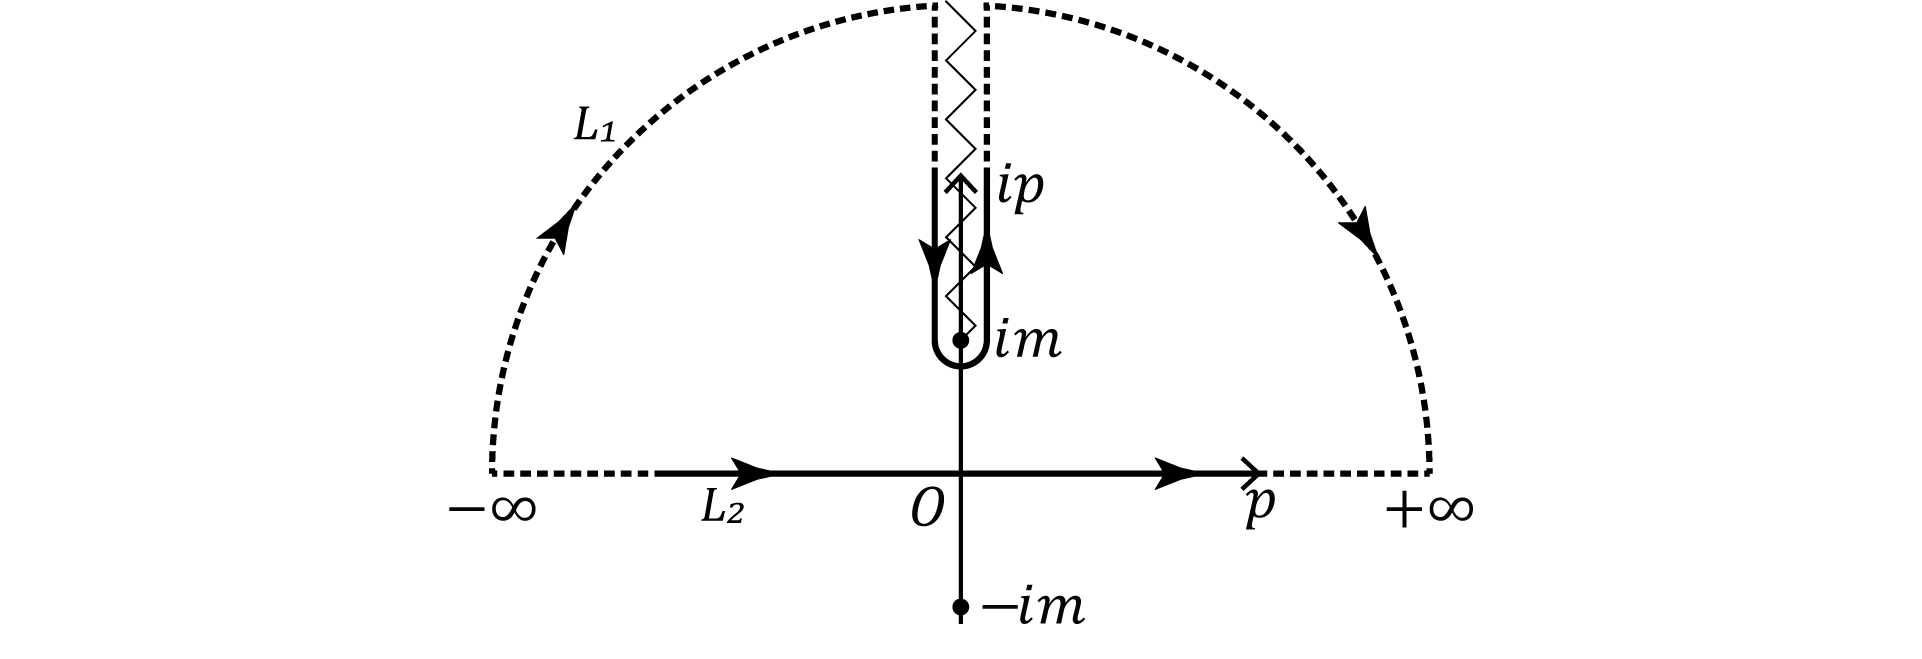
\includegraphics[width = 0.8\textwidth]{P27_2.52.png}
  \caption{Push contour}
  \label{fig: pushcon}
\end{figure}

因此, 若记
\begin{equation}
  f(p) = \frac{pe^{ipr}}{\sqrt{p^2+m^2}},
\end{equation}
并将$p$视为复数, 则有
\begin{equation}\label{eq: push_contour}
  \begin{aligned}
    \int_{L_2}dp\ f(p) & = \int_{L_1}dp\ fp                                  \\
                       & = \int_{\gamma_2}p\ f(p) + \int_{\gamma_1}dp\ f(p),
  \end{aligned}
\end{equation}
其中积分路径为
\begin{equation*}
  \begin{aligned}
    \gamma_1: p(\rho) = i\rho, \rho\in[m,+\infty], \\
    \gamma_2: p(\rho) = i\rho, \rho\in[+\infty,m],
  \end{aligned}
\end{equation*}
这里选择从上半平面积分是因为当$|p|\to\infty$时, $f(p)$在上半平面一致收敛为0.
因此, 两个无穷大$1/4$圆弧上积分值为0; 再考虑到$im$处无穷小半圆弧上的积分值为0, 我们就得到了笔记 \eqref{eq: push_contour} 式的第二行.

点$p = \pm im$是$\sqrt{p^2+m^2}$的支点(branch point).
从分支左侧到右侧时, 需要考虑图 \ref{fig: pushcon} 中所示的分支切割(branch cut), 此时$p^2+m^2$获得了$2\pi$的相位, 即$\sqrt{p^2+m^2}$获得了相位$e^{i\pi}$.
因此,
\begin{equation}
  \begin{aligned}
    \int_{L_2}dp\,f(p) & = \int_{\gamma_2}dp\,f(p) + \int_{\gamma_1}dp\,f(p)                     \\
                       & = \int_{\gamma_2}dp\,\frac{pe^{ipr}}{\sqrt{p^2+m^2}}
    + \int_{\gamma_1}dp\,\frac{pe^{ipr}}{e^{i\pi}\sqrt{p^2+m^2}}                                 \\
                       & = -2\int_{\gamma_1}dp\,\frac{pe^{ipr}}{\sqrt{p^2+m^2}}                  \\
                       & = 2i\int_{m}^{\infty}d\rho\,\frac{\rho e^{-\rho r}}{\sqrt{\rho^2-m^2}},
  \end{aligned}
\end{equation}
将积分结果带回即可得到书中(2.52)式.

\subsection{P28 - (2.53)}

这个commutator用此笔记的 \ref{subsubsec: Invar_Delta} 中的$\Delta$可以表示为:
\begin{equation}
  [\phi(x), \phi(y)] = i\Delta(x-y; m).
\end{equation}

\begin{mybox}{类空传播振幅不为零却不违反因果律}
  传播振幅并非可观测量, 而我们真正关心的是: 在$\mathbf{x}$处产生一个粒子会对在$\mathbf{y}$处产生一个粒子有什么影响, 所以需要计算算符对易关系$[\phi(x), \phi(y)]$.
\end{mybox}

\subsection{P30 - (2.54)}

第二行第二项的$e$指数项中除了把$E_\mathbf{p}$写为了$-(-E_\mathbf{p})$以外, 还做了变换$\mathbf{p} \rightarrow -\mathbf{p}$.

最后一步反着算比较容易: 在最后一行的式子中计算关于$p^0$的积分, 从下方闭合积分路径, 使用留数定理就可以得到第二行的表达式(最后一行表达式中的那个$(-1)$是因为从下方闭合了积分路径); 而这里当$(x_0 - y_0)>0$才从下方闭合积分路径的原因是只有这样$e^{-ip(x - y)}$才在无穷远处为零.

\subsection{P30 - (2.56)}

首先注意:
\begin{equation}
  \partial_\mu \theta(x^0) = g_{0\mu} \delta(x^0) \label{eq: partial_on_delta}.
\end{equation}

第一行: 对阶跃函数求一次导, 再应用分部积分后会得到
\begin{equation}
  \partial_0 \Bigl(\delta(x_0 - y_0)\langle 0|[\phi(x), \phi(y)]|0\rangle \Bigr)-\delta(x_0 - y_0)\partial_0\langle 0|[\phi(x), \phi(y)]|0\rangle,
\end{equation}
其中第一项等于0的原因可以粗略理解为: $x_0 \neq y_0$时, $\delta(x_0 - y_0)$等于0; $x_0 = y_0$时, $\langle 0|[\phi(x), \phi(y)]|0\rangle$等于0.

第二行: 注意使用此笔记的 \eqref{eq: partial_on_delta} 式及书中的(2.47).

第三行: Klein-Gordon equation.

\subsection{P30 - (2.57)}

给等式两边作用微分算符$(\partial^2 + m^2)$, 再比较两边的形式, 就可以得到(2.57)下面的表达式.

\subsection{P31 - (2.59)}

这里极点的计算有个小trick: 我们得到$p^0 = \pm\sqrt{E_\mathbf{p}^2 - i\epsilon}$后, 对小量$\epsilon$展开可得$p^0 = \pm (E_\mathbf{p} - \frac{1}{2}i\epsilon)$, 这时只要令$\epsilon^* = \frac{1}{2}\epsilon$即可(都是同阶无穷小).


  \pagestyle{general}
  \chapter{The Dirac Field}

\nonumsec{Summary}
\begin{itemize}
  \item \textbf{}整章内容都是基础, 需要掌握所有公式的推导
  \item \textbf{}书中第47页定义了螺度(helicity)算符
  \item \textbf{}书中第51页提到了轴矢量流和手征变换
  \item \textbf{}书中第48页写了旋量的具体表达式
  \item \textbf{}书中第72页关于\textbf{离散对称变换}的表可以帮助我们构建真实的粒子在场论中具体算符的形式(根据宇称等量子数)
  \item \textbf{}费曼传播子(\textbf{旋量场}):
        \begin{equation*}
          \langle 0|T\psi(x)\overline{\psi}(y)|0 \rangle = S_F(x-y)\equiv \int \frac{d^4 p}{(2\pi)^4} \frac{i(\cancel{p} + m)}{p^2 - m^2 +i\epsilon} e^{-ip\cdot (x-y)}
        \end{equation*}
        \begin{mybox}{另一种常见的写法}
          \begin{equation*}
            \tilde{S}_F(p) = \frac{i}{\cancel{p} - m +i\epsilon}
          \end{equation*}
        \end{mybox}
\end{itemize}
\pagestyle{general}

\section{Lorentz Invariance in Wave Equations}

注意: 本书中的变换都是对场本身进行操作. (\textit{active} point of view)

\subsection{P36 - (3.3)}

这里只要把$(\Lambda^{-1}x)$看作是$x$的某个函数$y(x) = \Lambda^{-1}x$, 做复合函数的求导即可.
等式右端最后那个括号的意思是前面的函数$\partial_{\nu}\phi$在$\Lambda^{-1}x$处取值.

\subsection{P39 - (3.15) (3.16)}

$J^3 = J^{12}$中, 3是(3.15)中的的上标, 12是中间没有序号的式子中的上标.

从这里开始会用全反对称的张量来表示矢量.
它们所带有的信息是一样的, 只是形式上对称的量会更方便使用.
而同时, 后面的参数也被全反对称化了, 也因此多了个$1/2$的系数.

\begin{mybox}{关于张量的计算}
  一开始学到这里的时候我很迷惑, 不过习惯了就好了.
  对这些含有张量的表达式或运算感到疑惑的时候, 把分量具体写出来算一遍总是个好办法.
\end{mybox}

\subsection{P39 - (3.17)}

我们在书中(3.16)这一具体表示下计算得到了Lorentz Algebra生成元之间的对易关系, 而由于代数本身与表示无关, 故书中(3.17)就是Lorentz Algebra的定义.
随后我们将使用此定义来计算Lorentz Algebra在其他空间中的具体表示.

\subsection{P39 - (3.18)}

这是洛伦兹群在矢量空间的具体表示, 相当重要, 后面也要用到.
$\mu\nu$指标代表着6个洛伦兹变换(3个boost和3个rotation), $\alpha$和$\beta$代表矢量的4个分量.

\begin{mybox}{区分空间指标}
  注意区分矢量空间和其他空间 (这一章基本是旋量空间) 的指标.
  一般后者会被省略.
\end{mybox}

关于它是怎么来的: 可以尝试在Minkowski时空中写出(3.16)的具体表示(把它作用到某个具体的时空$4$-vector上), 会得到一些和这个形式很像的东西! (正确的计算方法不是这样的, 但总之这个式子不完全是被\textit{pulled out of a hat} !)

\begin{mybox}{个人理解}
  可以尝试计算
  \begin{equation}
    \begin{aligned}
      x_\alpha & \rightarrow i(x^\mu\partial^\nu-x^\nu\partial^\mu)x_\beta                                                                                         \\
               & = i(x^\mu\delta^\nu_{\phantom{\nu}\beta} - x^\nu\delta^\mu_{\phantom{\mu}\beta})                                                                  \\
               & = i(\delta^\mu_{\phantom{\mu}\alpha} \delta^\nu_{\phantom{\nu}\beta} - \delta^\nu_{\phantom{\nu}\alpha} \delta^\mu_{\phantom{\mu}\beta})x^\alpha.
    \end{aligned}
  \end{equation}
\end{mybox}

\subsection{P40 - (3.19)}

写成有限形式就是$V' = \exp{(-\frac{i}{2}\omega_{\mu\nu}\mathcal{J}^{\mu\nu})}V$. (对比书中(3.13))

\section{The Dirac Equation}

狄拉克旋量具体可写为:
\begin{equation}
  \psi = \begin{pmatrix}
    \psi_1 \\ \psi_2 \\ \psi_3 \\ \psi_4
  \end{pmatrix},
\end{equation}
其狄拉克共轭为:
\begin{equation}
  \overline{\psi} = \psi^\dagger \gamma^0 = \Bigl(\psi^\dagger_1, \psi^\dagger_2, \psi^\dagger_3, \psi^\dagger_4\Bigr)\gamma^0.
\end{equation}

\subsection{P40 - (3.23)}

\begin{equation}
  \begin{aligned}
    \relax
    [S^{\mu\nu}, S^{\rho\sigma}] & = \biggl[\frac{i}{4}(\gamma^\mu \gamma^\nu - \gamma^\nu \gamma^\mu), \ \frac{i}{4}(\gamma^\rho \gamma^\sigma - \gamma^\sigma \gamma^\rho)\biggr]                                                                                           \\
                                 & = \biggl(\frac{i}{4}\biggr)^2 \Bigl\{\gamma^\mu \gamma^\nu \gamma^\rho \gamma^\sigma - \gamma^\mu \gamma^\nu \gamma^\sigma \gamma^\rho - \gamma^\nu \gamma^\mu \gamma^\rho \gamma^\sigma + \gamma^\nu \gamma^\mu \gamma^\sigma \gamma^\rho \\
                                 & \qquad \quad \ \ - \gamma^\rho \gamma^\sigma \gamma^\mu \gamma^\nu + \gamma^\rho \gamma^\sigma \gamma^\nu \gamma^\mu + \gamma^\sigma \gamma^\rho \gamma^\mu \gamma^\nu - \gamma^\sigma \gamma^\rho \gamma^\nu \gamma^\mu \Bigr\}.
  \end{aligned}
\end{equation}

注意到下面一行中上标的顺序恰好与上面一行的相反.
以第一项和最后一项为例子, 反复使用对易关系(3.22), 我们可以得到:
\begin{equation}
  \begin{aligned}
      & \gamma^\mu \gamma^\nu \gamma^\rho \gamma^\sigma - \gamma^\sigma \gamma^\rho \gamma^\nu \gamma^\mu                                                                                                                                          \\
    = & - 2g^{\mu\nu}\gamma^\sigma \gamma^\rho + 2g^{\mu\rho}\gamma^\sigma \gamma^\nu - 2g^{\mu\sigma}\gamma^\rho \gamma^\nu + 2g^{\nu\rho}\gamma^\mu \gamma^\sigma - 2g^{\nu\sigma}\gamma^\mu \gamma^\rho + 2g^{\rho\sigma}\gamma^\mu \gamma^\nu.
  \end{aligned}
\end{equation}
计算其余三项时调整上标即可(善用文本编辑器的\textbf{查找和替换}功能).

大括号内结果:
\begin{equation}
  \begin{aligned}
     & - 2g^{\mu\nu}\gamma^\sigma \gamma^\rho + 2g^{\mu\rho}\gamma^\sigma \gamma^\nu - 2g^{\mu\sigma}\gamma^\rho \gamma^\nu + 2g^{\nu\rho}\gamma^\mu \gamma^\sigma - 2g^{\nu\sigma}\gamma^\mu \gamma^\rho + 2g^{\rho\sigma}\gamma^\mu \gamma^\nu  \\
     & + 2g^{\mu\nu}\gamma^\rho \gamma^\sigma - 2g^{\mu\sigma}\gamma^\rho \gamma^\nu + 2g^{\mu\rho}\gamma^\sigma \gamma^\nu - 2g^{\nu\sigma}\gamma^\mu \gamma^\rho + 2g^{\nu\rho}\gamma^\mu \gamma^\sigma - 2g^{\sigma\rho}\gamma^\mu \gamma^\nu  \\
     & + 2g^{\nu\mu}\gamma^\sigma \gamma^\rho - 2g^{\nu\rho}\gamma^\sigma \gamma^\mu + 2g^{\nu\sigma}\gamma^\rho \gamma^\mu - 2g^{\mu\rho}\gamma^\nu \gamma^\sigma + 2g^{\mu\sigma}\gamma^\nu \gamma^\rho - 2g^{\rho\sigma}\gamma^\nu \gamma^\mu  \\
     & - 2g^{\nu\mu}\gamma^\rho \gamma^\sigma + 2g^{\nu\sigma}\gamma^\rho \gamma^\mu - 2g^{\nu\rho}\gamma^\sigma \gamma^\mu + 2g^{\mu\sigma}\gamma^\nu \gamma^\rho - 2g^{\mu\rho}\gamma^\nu \gamma^\sigma + 2g^{\sigma\rho}\gamma^\nu \gamma^\mu,
  \end{aligned}
\end{equation}
消项合并后可以得到:
\begin{equation}
  -4g^{\mu\rho}[\gamma^\nu, \gamma^\sigma] + 4g^{\mu\sigma}[\gamma^\nu, \gamma^\rho] + 4g^{\nu\rho}[\gamma^\mu, \gamma^\sigma] - 4g^{\nu\sigma}[\gamma^\mu, \gamma^\rho],
\end{equation}
考虑系数$(\frac{i}{4})^2$, 即可证明(3.23)满足(3.17).

\subsection{P42 - (3.28)下面的两个式子}

第一个式子的证明:
\begin{equation}
  \begin{aligned}
    l.h.s & = \frac{i}{4}\bigl[\gamma^\mu, [\gamma^\rho, \gamma^\sigma]\bigr]                                                                                                                                  \\
          & = \frac{i}{4}[\gamma^\mu, \gamma^\rho \gamma^\sigma] - \frac{i}{4}[\gamma^\mu, \gamma^\sigma \gamma^\rho]                                                                                          \\
          & = \frac{i}{4}\Bigl(\{\gamma^\mu, \gamma^\rho\}\gamma^\sigma - \gamma^\rho\{\gamma^\mu, \gamma^\sigma\} - \{\gamma^\mu, \gamma^\sigma\}\gamma^\rho + \gamma^\sigma\{\gamma^\mu, \gamma^\rho\}\Bigr) \\
          & = \frac{i}{4}\Bigl(2g^{\mu\rho}\gamma^\sigma - 2g^{\mu\sigma}\gamma^\rho - 2g^{\mu\sigma}\gamma^\rho + 2g^{\mu\rho}\gamma^\sigma                                                                   \\
          & = i(g^{\mu\rho}\gamma^\sigma - g^{\mu\sigma}\gamma^\rho),                                                                                                                                          \\
    \                                                                                                                                                                                                          \\
    r.h.s & = g^{\mu\lambda}(\mathcal{J}^{\rho\sigma})_{\lambda\nu} \gamma^\nu                                                                                                                                 \\
          & = g^{\mu\lambda}\cdot i(\delta^\rho_{\phantom{1}\lambda} \delta^\sigma_{\phantom{1}\nu} - \delta^\rho_{\phantom{1}\nu} \delta^\sigma_{\phantom{1}\lambda}) \gamma^\nu                              \\
          & = i(g^{\mu\rho}\gamma^\sigma - g^{\mu\sigma}\gamma^\rho),
  \end{aligned}
\end{equation}
$l.h.s = r.h.s$, 即证.

第二个式子中, 把左边展开后忽略二阶小量即可.

\subsection{P42 - (3.31)下方验证洛伦兹协变的式子}

对第一行的$\gamma^\mu \partial_\mu$做变换后会多出来一个$\Lambda^{-1}$的原因参考书中式(3.3).

\subsection{P43 - (3.35)}

小技巧:
\begin{equation}
  \frac{\partial (\partial_\mu \phi)}{\partial (\partial_\nu \phi)} = \delta_\mu^{\phantom{1}\nu},
\end{equation}
相似地,
\begin{equation}
  \frac{\partial (\partial_\mu A_\nu)}{\partial (\partial_\rho A_\sigma)} = \delta_\mu^{\phantom{1}\rho}\delta_\nu^{\phantom{1}\sigma}.
\end{equation}

\subsection{P44 - (3.38)}

注意这里的$\sigma^2$指$\sigma^i, i=2$.
(我第一次遇见的时候以为是$\bm{\sigma}$的平方, $\bm{\sigma}^2$, 想了好半天)

\section{Free-Particle Solutions of the Dirac Equation}

\subsection{P46 - (3.49)}\label{subsubsec: Boost_u_p}

\begin{enumerate}
  \item \textbf{}最后一步要用到(3.48)的结果, 即$\sqrt{m}\ e^{\eta/2} = \sqrt{E + p^3}$, 以及$\sqrt{m}\ e^{-\eta/2} = \sqrt{E - p^3}$.
  \item \textbf{}若只考虑3-direction, 最终结果可以写为
        \begin{equation}
          \begin{pmatrix}
            \biggl(\begin{smallmatrix}
                     \sqrt{E-p^3} & 0 \\ 0 & \sqrt{E+p^3}
                   \end{smallmatrix}\biggr)\xi \\
            \biggl(\begin{smallmatrix}
                     \sqrt{E+p^3} & 0 \\ 0 & \sqrt{E-p^3}
                   \end{smallmatrix}\biggr)\xi
          \end{pmatrix},
        \end{equation}
  \item \textbf{}这里对$u(p_0)$进行boost后得到了$u(p)$, 完整形式实际上是$u'(\Lambda p_0) = \Lambda_{\frac{1}{2}}u(p_0)$ (boost后应有prime), 即$u'(p) = \Lambda_{\frac{1}{2}}u(\Lambda^{-1}p)$, 与书中(3.8)式形式一致.
        (在推导(3.110)时会用到)
        \begin{mybox}{}
          书中(3.8)是坐标空间下的变换规则, 但按照书中(3.2)式的思想, 动量空间中的变换规则也应该是一致的.
          最直接的验证方法是将书中(3.46)式($u(p)$为满足此方程的解)写为$(\gamma^\mu(\Lambda p)_\mu - m)u(\Lambda p) = 0$, 利用书中(3.29)式得到含有$\Lambda_{1/2}$的形式后, 再和原式做比较.

          \mbox{}

          附另外一个直接推导:

          由于$\psi(x) = u(p)e^{-ip\cdot x}$, 所以进行变换$\psi(x) \rightarrow \psi'(x) = \Lambda_{\frac{1}{2}}\psi(\Lambda^{-1}x)$后, 对$u(p)$有
          \begin{equation}
            \begin{aligned}
              u'(p)e^{-ip\cdot x} & = \Lambda_{\frac{1}{2}}u(p)e^{-ip\cdot \Lambda^{-1}x}                           \\
              u'(p)e^{-ip\cdot x} & = \Lambda_{\frac{1}{2}}u(\Lambda^{-1}p')e^{-i\Lambda^{-1}p'\cdot \Lambda^{-1}x} \\
              u'(p)e^{-ip\cdot x} & = \Lambda_{\frac{1}{2}}u(\Lambda^{-1}p')e^{-ip'\cdot x},
            \end{aligned}
          \end{equation}
          所以对$\psi(x)$的做的变换实际上使得
          \begin{equation}
            u(p) \rightarrow u'(p) = \Lambda_{\frac{1}{2}}u(\Lambda^{-1}p).
          \end{equation}
        \end{mybox}
\end{enumerate}

\subsection{P46 - (3.50)}

\begin{enumerate}
  \item \textbf{}关于$\sqrt{p\cdot \sigma}$的含义:

        在只考虑3-direction时, $p\cdot \sigma = p^0 + p^3\sigma^3$, 已经是对角化的形式, 取正根即可.

        若考虑更一般的形式, 对(3.49)式的结果做替换$\sigma^3 \rightarrow \bm{\sigma}\cdot\hat{n},\ p^3 \rightarrow \mathbf{p}\cdot\hat{n}$, 其中$\hat{n} = \hat{p}$.
        考虑第一个分量的平方
        \begin{equation}
          \begin{aligned}
              & \biggl(\sqrt{E+\mathbf{p}\cdot\hat{n}} \frac{1-\bm{\sigma}\cdot\hat{n}}{2} + \sqrt{E-\mathbf{p}\cdot\hat{n}} \frac{1+\bm{\sigma}\cdot\hat{n}}{2} \biggr)^2                        \\
            = & (E+\mathbf{p}\cdot\hat{n}) \frac{1-\bm{\sigma}\cdot\hat{n}}{2} + (E-\mathbf{p}\cdot\hat{n}) \frac{1+\bm{\sigma}\cdot\hat{n}}{2} + \sqrt{E^2 - (\mathbf{p}\cdot\hat{n})^2} \cdot 0 \\
            = & E - (\mathbf{p}\cdot\hat{n})(\bm{\sigma}\cdot\hat{n})                                                                                                                             \\
            = & E - \mathbf{p} \cdot \bm{\sigma}                                                                                                                                                  \\
            = & p \cdot \sigma .
          \end{aligned}
        \end{equation}
  \item \textbf{}本书的\href{https://www.slac.stanford.edu/~mpeskin/QFT.html}{纠错网页}提到旋量$u(p)$还可以被表示为:
        \begin{equation}\label{eq: spinor_explicit(ch.3)}
          u(p)=\begin{pmatrix}
            \frac{p\cdot \sigma + m}{\sqrt{2(E+m)}}\xi \\
            \frac{p\cdot \bar{\sigma} + m}{\sqrt{2(E+m)}}\xi
          \end{pmatrix}
        \end{equation}

        证明:
        \begin{equation}
          \begin{aligned}
            \biggl(\frac{p\cdot \sigma + m}{\sqrt{2(E+m)}}\biggr)^2 & = \frac{1}{2(E+m)}(E-\mathbf{p}\cdot \bm{\sigma}+m)^2                                                                                                    \\
                                                                    & = \frac{1}{2(E+m)}(E^2 - 2E\ \mathbf{p}\cdot \bm{\sigma} + (\mathbf{p}\cdot \bm{\sigma})^2 + 2mE - 2m\ \mathbf{p}\cdot \bm{\sigma} + E^2 - \mathbf{p}^2) \\
                                                                    & = \frac{1}{2(E+m)} (2E(E + m) - 2\mathbf{p}\cdot \bm{\sigma}(E + m))                                                                                     \\
                                                                    & = (E - \mathbf{p}\cdot \bm{\sigma}) = p\cdot \sigma.
          \end{aligned}
        \end{equation}
        注意其中$(\mathbf{p}\cdot \bm{\sigma})^2 = \mathbf{p}^2$.
        $(p\cdot \bar{\sigma} + m)$一项的证明也是类似的.

        又注意到
        \begin{equation}
          u(p)=\begin{pmatrix}
            \frac{p\cdot \sigma + m}{\sqrt{2(E+m)}}\xi \\
            \frac{p\cdot \bar{\sigma} + m}{\sqrt{2(E+m)}}\xi
          \end{pmatrix}
          =\frac{1}{\sqrt{2m(E+m)}}\begin{pmatrix}
            m                   & p\cdot \sigma \\
            p\cdot \bar{\sigma} & m
          \end{pmatrix}
          \sqrt{m}
          \begin{pmatrix}
            \xi \\
            \xi
          \end{pmatrix},
        \end{equation}
        于是
        \begin{equation}
          u(p) = \frac{\cancel{p}+m}{\sqrt{2m(E+m)}}u(p_0).
        \end{equation}
\end{enumerate}

\subsection{P46 - (3.51)}

记得把(3.50)代回到(3.45)后再做计算.

\subsection{P47 - (3.54)}
当粒子的动量方向沿着$3$-direction时, $h = \hat{p}_3\cdot S_3=\frac{1}{2}\sigma_3$, (3.52)和(3.53)自然是其本征态(它们都是考虑沿着$3$-direction的boost得到的具体表达).

\begin{mybox}{评论}
  \begin{enumerate}
    \item 在(3.52)和(3.53)中的large boost意味着我们考虑了$m\rightarrow 0$的情况($E^2 = \mathbf{p}^2 + m^2$), 而无质量极限下的Dirac旋量场满足Weyl equations(书中(3.40)式).
          此时我们发现, Dirac旋量的具体表示也“恰好”变成了Weyl旋量的形式, 即
          \begin{equation}
            \left\{\begin{array}{l}
              \psi_L = \sqrt{2E}\ e^{-ip\cdot x} \bigl(\begin{smallmatrix} 0 \\ 1 \end{smallmatrix}\bigr) \\
              \psi_R = \sqrt{2E}\ e^{-ip\cdot x} \bigl(\begin{smallmatrix} 1 \\ 0 \end{smallmatrix}\bigr)
            \end{array}\right.,
          \end{equation}
          并且它们有着定义良好的螺度本征值.
    \item 其实我们从书中(3.40)式就可以发现Weyl旋量是螺度算符的本征态(以$\psi_L$为例):
          \begin{equation}
            i(\partial_0 - \bm{\sigma}\cdot \bm{\nabla})\psi_L = i\partial_0 u(p)e^{-ip\cdot x} + i(\bm{\sigma}\cdot \bm{\nabla}) u(p)e^{-ip\cdot x} = 0,
          \end{equation}
          即
          \begin{equation}
            (\bm{\sigma} \cdot \mathbf{p})\psi_L = -E\psi_L,
          \end{equation}
          化简后即为$(\hat{p}\cdot \bm{\sigma})\psi_L = -\psi_L$(注意$m\rightarrow 0$, 即$|\mathbf{p}|\rightarrow E$).
          $\psi_R$同理.
    \item 如果在书中(3.47)不加入$\sqrt{m}$这个系数, 无质量极限下旋量的具体表示会在分母上有个$\sqrt{m}$, 从而导致表达式发散.
  \end{enumerate}
\end{mybox}

\section{Dirac Matrices and Dirac Field Bilinears}

\subsection{P50 - (3.72)}

这里可以自己验证一下$\bar{\psi} \gamma^5 \psi$在连续洛伦兹变换下是标量.

\subsection{P51 - (3.76)}

利用书中(3.72),
\begin{equation}
  \biggl( \frac{1 - \gamma^5}{2} \biggr) \psi = \begin{pmatrix}
    1 & 0 \\
    0 & 0
  \end{pmatrix}
  \begin{pmatrix}
    \psi_L \\
    \psi_R
  \end{pmatrix} = \begin{pmatrix}
    \psi_L \\
    0
  \end{pmatrix},
\end{equation}
而$\psi^\dagger \gamma^0 \gamma^\mu$中的两个$\gamma$相乘会得到对角形式的矩阵.
因此整个表达式只与$\psi_L$有关, 为左手流.

\subsection{P51 - (3.77)}

建议对16个分量直接进行验证.

\subsection{P51 - (3.78)}

将矩阵的元素(即带有下标的形式, 例如$\epsilon_{\alpha \gamma}$)具体写出来后, 由于这些元素只是数字(\textit{c-number}), 所以可以随便挪动位置.
(矩阵乘法的分量形式: $(AB)_{ab} = \sum_c A_{ac} B_{cb}$) 后面的计算中经常要用到这个技巧.

恒等式的证明:
\begin{equation}
  \begin{aligned}
    l.h.s. & = (\bar{u}_{1R})_\alpha (u_{2R})_\beta (\bar{u}_{3R})_\gamma (u_{4R})_\delta (\sigma^{\mu})_{\alpha\beta} (\sigma_{\mu})_{\gamma\delta}      \\
           & = (\bar{u}_{1R})_\alpha (u_{2R})_\beta (\bar{u}_{3R})_\gamma (u_{4R})_\delta (2\epsilon_{\alpha\gamma} \epsilon_{\beta\delta})               \\
           & = (\bar{u}_{1R})_\alpha (u_{2R})_\beta (\bar{u}_{3R})_\gamma (u_{4R})_\delta (-2\epsilon_{\alpha\gamma} \epsilon_{\delta\beta})              \\
           & = (\bar{u}_{1R})_\alpha (u_{2R})_\beta (\bar{u}_{3R})_\gamma (u_{4R})_\delta (\sigma^{\mu})_{\alpha\delta} (\sigma_{\mu})_{\gamma\beta} (-1) \\
           & = -(\bar{u}_{1R} \sigma^{\mu} u_{4R})(\bar{u}_{3R} \sigma_{\mu} u_{2R}),
  \end{aligned}
\end{equation}
第三行中调换了$\beta$和$\delta$的位置.

\section{Quantization of the Dirac Field}

\subsection{{P52} - (3.84)}
\begin{equation}
  \begin{aligned}
    \mathcal{H} & = i {\psi}^\dagger \dot{\psi} - \mathcal{L}                                                              \\
                & = i {\psi}^\dagger \dot{\psi} - i \bar{\psi} \gamma^0 \dot{\psi} - i \bar{\psi} \gamma^i \partial_i \psi \\
                & = {\psi}^\dagger (-i \gamma^i \partial_i + m) \psi.
  \end{aligned}
\end{equation}

\begin{mybox}{}
  注意$\gamma^\mu \partial_\mu = \gamma^0 \partial_0 + \gamma^i \partial_i$
  不要习惯性地写成减号.
\end{mybox}

\subsection{P52 - (3.86)}
为什么在标量场部分我们关心的是场和其正则动量的对易关系, 而在这里我们关心的是$\psi$和$\bar{\psi}$的对易关系呢?

小提示: 尝试计算一下它们的正则动量! (Peskin \& Schroeder你们明说一下多好\ 〒\_〒)

\subsection{P54 - (3.90)}

利用$u^s(\mathbf{p})e^{i\mathbf{p} \cdot \mathbf{x}}$是$h_D$的本征函数的性质简化书中(3.84), 之后的计算很简单.

\subsection{P59 - (3.110)附近}
\begin{enumerate}
  \item \textbf{}注意$p\cdot x = \Lambda p\cdot \Lambda x$(书中(3.4)式).
  \item \textbf{}(3.110)上面一行里的那个关系在此笔记的 \ref{subsubsec: Boost_u_p} 中已经证明过了.
\end{enumerate}

\section{Discrete Symmetries of the Dirac Theory}

\subsection{P67 - 中间没有序号的式子}

这里是说$\psi(-t, \mathbf{x})|0\rangle$应该是正频项的和$e^{-iHt}\psi(\mathbf{x})|0\rangle$, 但用时间反演算符计算得到的结果却是负频项的和$e^{iHt}[T\psi(\mathbf{x})T]|0\rangle$.
它们之间是矛盾的.

\subsection{P68 - (3.134)}

$\xi(\uparrow)$和$\xi(\downarrow)$是$\bm{\sigma}\cdot\mathbf{\hat{n}}$的本征态.
参见\textit{Modern Quantum Mechanics - J.J.Sakurai}: \textbf{Problem 1.9}.

\subsection{P68 - (3.136)}

这里可以把$\eta^s$写为$\xi^{-s}$的原因在(3.112)上面的那一大段话中有讲.

\subsection{P70 - (3.147)}

关于这里第三步中出现的负号, 具体计算过程如下:
\begin{equation*}
  \begin{aligned}
    -\gamma^0_{ab}\gamma^2_{bc}\psi_c\bar{\psi}_d\gamma^0_{de}\gamma^2_{ea} = & +\bar{\psi}_d \gamma^0_{de}\gamma^2_{ea}\gamma^0_{ab}\gamma^2_{bc}\psi_c - \bigl\{\psi_c,\psi_f^\dagger\bigr\}\gamma^0_{fd} \gamma^0_{ab}\gamma^2_{bc}\gamma^0_{de}\gamma^2_{ea}\ ,
  \end{aligned}
\end{equation*}
其中第二项为(第三行用到了奇数个$\gamma^{\mu}$矩阵的迹为零的性质)
\begin{equation*}
  \begin{aligned}
    \bigl\{\psi_c,\psi_f^\dagger\bigr\}\gamma^0_{fd} \gamma^0_{ab}\gamma^2_{bc}\gamma^0_{de}\gamma^2_{ea} = & \delta_{cf}\gamma^0_{fd}\gamma^0_{ab}\gamma^2_{bc}\gamma^0_{de}\gamma^2_{ea}\delta^{(3)}(\mathbf{x}-\mathbf{x}) \\
    =                                                                                                       & \mathrm{Tr}\bigl(\gamma^0 \gamma^0 \gamma^2 \gamma^0 \gamma^2\bigr)\delta^{(3)}(0)                              \\
    =                                                                                                       & 0 \delta^{(3)}(0)                                                                                               \\
    =                                                                                                       & 0.
  \end{aligned}
\end{equation*}
故
\begin{equation*}
  \begin{aligned}
    -\gamma^0_{ab}\gamma^2_{bc}\psi_c\bar{\psi}_d\gamma^0_{de}\gamma^2_{ea} = & +\bar{\psi}_d \gamma^0_{de}\gamma^2_{ea}\gamma^0_{ab}\gamma^2_{bc}\psi_c.
  \end{aligned}
\end{equation*}

\clearpage
\nonumsec{Problems}
\nonumssec{3.1 Lorentz group}
\paragraph*{(1)定义:}
\begin{itemize}
  \item \textbf{Lorentz algebra}
        \begin{equation}
          [J^{\mu\nu}, J^{\rho\sigma}] = i(g^{\nu\rho}J^{\mu\sigma} - g^{\mu\rho}J^{\nu\sigma} - g^{\nu\sigma}J^{\mu\rho} + g^{\mu\sigma}J^{\nu\rho}).
        \end{equation}
  \item \textbf{Generators of rotations and boosts}
        \begin{equation}
          L^i = \tfrac{1}{2}\epsilon^{ijk}J^{jk},\qquad K^i = J^{0i}.
        \end{equation}
  \item \textbf{Lorentz transformation}

        无穷小变换可以写为:
        \begin{equation}
          \Phi \rightarrow (1 - i\bm{\theta}\cdot\mathbf{L} - i\bm{\beta}\cdot\mathbf{K})\Phi.
        \end{equation}

        如果定义$\theta_i = \epsilon_{ijk}\omega_{jk}$, $\beta_i = \omega_{0i}$, 则Lorentz transformation可以简略地表示为
        \begin{equation}
          \Lambda = \exp(-\tfrac{i}{2}\omega_{\mu\nu}J^{\mu\nu}).
        \end{equation}
  \item \textbf{Decomposition of the group}
        \begin{equation}
          \mathbf{J}_+ = \tfrac{1}{2}(\mathbf{L}+i\mathbf{K})\ \ \ {\rm and}\ \ \ \mathbf{J}_- = \tfrac{1}{2}(\mathbf{L}-i\mathbf{K}).
        \end{equation}
\end{itemize}

\paragraph*{(2)计算对易关系: }
\begin{itemize}
  \item $[L^i, L^j]$
        \begin{equation}
          \begin{aligned}
            \relax[L^i, L^j] & = [\tfrac{1}{2}\epsilon^{ikl}J^{kl}, \tfrac{1}{2}\epsilon^{jmn}J^{mn}]                                \\
                             & = \tfrac{i}{4}\epsilon^{ikl}\epsilon^{jmn}(g^{lm}J^{kn} - g^{km}J^{ln} - g^{ln}J^{km} + g^{kn}J^{lm}) \\
                             & = i\epsilon^{ikl}\epsilon^{jmn}\delta^{km}J^{ln}                                                      \\
                             & = i\epsilon^{kil}\epsilon^{kjn}J^{ln}                                                                 \\
                             & = i(\delta^{ij}\delta^{ln}-\delta^{in}\delta^{lj})J^{ln}                                              \\
                             & = i\delta^{ij}{\rm tr}(J) - iJ^{ji}                                                                   \\
                             & = \tfrac{1}{2}i(J^{ij} - J^{ji})                                                                      \\
                             & = \tfrac{1}{2}i(\delta^{im}\delta^{jn}-\delta^{in}\delta^{jm})J^{mn}                                  \\
                             & = \tfrac{1}{2}i\epsilon^{kij}\epsilon^{kmn}J^{mn}                                                     \\
                             & = i\epsilon^{ijk}L^k.
          \end{aligned}
        \end{equation}
        \begin{itemize}
          \item 行2 $\rightarrow$ 行3:

                \quad ①\ 对每一项, 调整上标位置后重新标记上标字母;

                \quad ②\ 由于$k, m = 1, 2, 3$, $g^{km} = -\delta^{km}$.
          \item 行4 $\rightarrow$ 行5 \& 行8 $\rightarrow$ 行9:

                \quad \ $\epsilon^{ijk}\epsilon^{imn} = \delta^{jm}\delta^{kn} - \delta^{jn}\delta^{km}$.
          \item 行6 $\rightarrow$ 行7: $J$ 全反对称; ${\rm tr}(J)=0$.
        \end{itemize}
  \item $[K^i, K^j]$
        \begin{equation}
          \begin{aligned}
            \relax[K^i, K^j] & = [J^{0i}, J^{0j}]                                             \\
                             & = i(g^{i0}J^{0j} - g^{00}J^{ij} - g^{ij}J^{00} + g^{0j}J^{i0}) \\
                             & = -iJ^{ij} = -i\epsilon^{ijk}L^k.
          \end{aligned}
        \end{equation}
  \item $[L^i, K^j]$
        \begin{equation}
          \begin{aligned}
            \relax[L^i, K^j] & = [\tfrac{1}{2}\epsilon^{ikl}J^{kl}, J^{0j}]                                            \\
                             & = \tfrac{i}{2}\epsilon^{ikl}(g^{l0}J^{kj} - g^{k0}J^{lj} - g^{lj}J^{k0} + g^{kj}J^{l0}) \\
                             & = \tfrac{i}{2}(\epsilon^{ikj}J^{k0} - \epsilon^{ijl}J^{j0})                             \\
                             & = i\epsilon^{ijk}J^{0k} = i\epsilon^{ijk}K^{k}.
          \end{aligned}
        \end{equation}
  \item $[\mathbf{J}_+, \mathbf{J}_-]$
        \begin{equation}
          \begin{aligned}
            \relax[\mathbf{J}_+, \mathbf{J}_-] & = [\tfrac{1}{2}(\mathbf{L}+i\mathbf{K}), \tfrac{1}{2}(\mathbf{L}-i\mathbf{K})] \\
                                               & = \tfrac{i}{4} (-[\mathbf{L}, \mathbf{K}] + [\mathbf{K}, \mathbf{L}])          \\
                                               & = -\tfrac{i}{2} \sum\nolimits_i [L^i, K^i]                                     \\
                                               & = \tfrac{1}{2}\sum\nolimits_i\epsilon^{iik}K^k = 0.
          \end{aligned}
        \end{equation}
  \item $[J_+^i, J_+^j]$ and $[J_-^i, J_-^j]$
        \begin{equation}
          \begin{aligned}
            \relax[J_+^i, J_+^j] & = [\tfrac{1}{2}(L^i+iK^i), \tfrac{1}{2}(L^j+iK^j)]                   \\
                                 & = \tfrac{1}{4}([L^i, L^j]+i[L^i, K^j]-i[L^j, K^i]-[K^i, K^j])        \\
                                 & = \tfrac{1}{4}i\epsilon^{ijk}(L^k + iK^k + iK^k + L^k)               \\
                                 & = i\epsilon^{ijk}\cdot\tfrac{1}{2}(L^k+iK^k) = i\epsilon^{ijk}J_+^k.
          \end{aligned}
        \end{equation}

        同理, $[J_-^i, J_-^j] = i\epsilon^{ijk}J_-^k$.
  \item \textbf{总结}:
        \begin{equation}
          \left\{\begin{array}{l}
            \relax[L^i, L^j] = i\epsilon^{ijk}L^k  \\
            \relax[K^i, K^j] = -i\epsilon^{ijk}L^k \\
            \relax[L^i, K^j] = i\epsilon^{ijk}K^k
          \end{array} \right.
        \end{equation}
        \begin{equation}{\label{eq: subalgebra_Lorentz}}
          \left\{\begin{array}{l}
            \relax[J_+^i, J_+^j] = i\epsilon^{ijk}J_+^k \\
            \relax[J_-^i, J_-^j] = i\epsilon^{ijk}J_-^k \\
            \relax[\mathbf{J}_+, \mathbf{J}_-] = 0
          \end{array} \right.
        \end{equation}
\end{itemize}

\paragraph*{(3)Decompose Lorentz Algebra: }
由上面的 \eqref{eq: subalgebra_Lorentz} 式可知, 洛伦兹代数可以被分解为两个${\rm su}(2)$子代数的直和, 即
\begin{equation}
  {\rm so}(1, 3) = {\rm su}(2) \bigoplus {\rm su}(2),
\end{equation}
而${\rm su}(2)$子代数的不可约表示是由一个角动量量子数$j$(取整数或半整数)来标记的, 故我们可以很方便地用一对整/半整数$(j_+, j_-)$来标记洛伦兹代数的所有不可约表示.

\paragraph*{(4) $(\frac{1}{2}, 0)$及$(0, \frac{1}{2})$表示: }
\begin{itemize}
  \item $(\frac{1}{2}, 0)$:
        \begin{equation}
          \left\{\begin{array}{l}
            \mathbf{J}_+ = \tfrac{1}{2}\bm{\sigma} \\
            \mathbf{J}_- = 0
          \end{array} \right.,
        \end{equation}
        则
        \begin{equation}
          \left\{\begin{array}{l}
            \mathbf{L} = \mathbf{J}_+ + \mathbf{J}_- = \frac{1}{2}\bm{\sigma} \\
            \mathbf{K} = -i(\mathbf{J}_+ - \mathbf{J}_-) = -\frac{i}{2}\bm{\sigma}
          \end{array} \right..
        \end{equation}
        无穷小变换可以写为
        \begin{equation}
          \Phi \rightarrow (1 - i\bm{\theta}\cdot\tfrac{\bm{\sigma}}{2} - \bm{\beta}\cdot\tfrac{\bm{\sigma}}{2})\Phi,
        \end{equation}
        对应$\psi_L$(左手Weyl spinor).
  \item $(0, \frac{1}{2})$:
        \begin{equation}
          \left\{\begin{array}{l}
            \mathbf{J}_+ = 0 \\
            \mathbf{J}_- = \tfrac{1}{2}\bm{\sigma}
          \end{array} \right.,
        \end{equation}
        则
        \begin{equation}
          \left\{\begin{array}{l}
            \mathbf{L} = \mathbf{J}_+ + \mathbf{J}_- = \frac{1}{2}\bm{\sigma} \\
            \mathbf{K} = -i(\mathbf{J}_+ - \mathbf{J}_-) = \frac{i}{2}\bm{\sigma}
          \end{array} \right..
        \end{equation}
        无穷小变换可以写为
        \begin{equation}
          \Phi \rightarrow (1 - i\bm{\theta}\cdot\tfrac{\bm{\sigma}}{2} + \bm{\beta}\cdot\tfrac{\bm{\sigma}}{2})\Phi,
        \end{equation}
        对应$\psi_R$(右手Weyl spinor).
\end{itemize}

\paragraph*{(5) 矢量表示: }
构造场$\psi'=\psi^T_L \sigma^2$, 对其作无穷小洛伦兹变换有
\begin{equation}
  \psi' \rightarrow \psi'(1 + i\bm{\theta}\cdot\tfrac{\bm{\sigma}}{2} + \bm{\beta}\cdot\tfrac{\bm{\sigma}}{2}).
\end{equation}
构造复合场$\Psi = \psi_R \psi'$, 则$\Psi$是一个满足洛伦兹群$(\frac{1}{2}, \frac{1}{2})$表示的$2\times 2$矩阵, 即
\begin{equation}
  \Psi \rightarrow (1 - i\bm{\theta}\cdot\tfrac{\bm{\sigma}}{2} + \bm{\beta}\cdot\tfrac{\bm{\sigma}}{2}) \Psi (1 + i\bm{\theta}\cdot\tfrac{\bm{\sigma}}{2} + \bm{\beta}\cdot\tfrac{\bm{\sigma}}{2}).
\end{equation}
将这个$2\times 2$矩阵参数化为$\Psi = \bar{\sigma}_{\mu}V^{\mu} = V^0 + \sigma^i V^i$, 即
\begin{equation}
  \Psi = \begin{pmatrix}
    V^0+V^3  & V^1-iV^2 \\
    V^1+iV^2 & V^0-V^3
  \end{pmatrix},
\end{equation}
变换关系可以写为
\begin{equation}
  \begin{aligned}
    \Psi & \rightarrow \begin{pmatrix}
                         1 + \frac{1}{2}(-i\theta^3+\beta^3)                     & \frac{1}{2}(-i\theta^1 - \theta^2 + \beta^1 - i\beta^2) \\
                         \frac{1}{2}(-i\theta^1 + \theta^2 + \beta^1 + i\beta^2) & 1 + \frac{1}{2}(i\theta^3-\beta^3)
                       \end{pmatrix}             \\
         & \quad\ \times \begin{pmatrix}
                           V^0+V^3  & V^1-iV^2 \\
                           V^1+iV^2 & V^0-V^3
                         \end{pmatrix}
    \begin{pmatrix}
      1 + \frac{1}{2}(i\theta^3+\beta^3)                     & \frac{1}{2}(i\theta^1 + \theta^2 + \beta^1 - i\beta^2) \\
      \frac{1}{2}(i\theta^1 - \theta^2 + \beta^1 + i\beta^2) & 1 - \frac{1}{2}(i\theta^3+\beta^3)
    \end{pmatrix}                                  \\
         & = \Psi + \begin{pmatrix}
                      \begin{matrix}
        \beta^3 V^0 + \beta^3 V^3 \\ + (- \theta^2 + \beta^1) V^1 + (\theta^1 + \beta^2) V^2
      \end{matrix}
                       &
                      \begin{matrix}
        (\beta^1 - i\beta^2) V^0 + (i\theta^1 + \theta^2) V^3 \\ -i\theta^3 V^1 - \theta^3 V^2
      \end{matrix}
                      \\ \mbox{} \\
                      \begin{matrix}
        (\beta^1 + i\beta^2) V^0 + (-i\theta^1 + \theta^2) V^3 \\ i\theta^3 V^1 - \theta^3 V^2
      \end{matrix}
                       &
                      \begin{matrix}
        -\beta^3 V^0 + \beta^3 V^3 \\ + (\theta^2 + \beta^1) V^1 + (-\theta^1 + \beta^2) V^2
      \end{matrix}
                    \end{pmatrix}                                                                                                        \\
         & = \Psi + \mathbf{1} \cdot \beta^i V^i + \sigma_1 (\beta^1 V^0 + \theta^2 V^3 - \theta^3 V^2)                                              \\
         & \qquad\ + \sigma_2 (\beta^2 V^0 -\theta^1 V^3 + \theta^3 V^1) + \sigma_3 (\beta^3 V^0 + \theta^1 V^2 - \theta^2 V^1)                      \\
         & = \Psi + \mathbf{1} \cdot \omega^{0j} V^j - \sigma_1 (\omega^{10}V^0 + \omega^{13}V^3 + \omega^{12}V^2)                                   \\
         & \qquad\ - \sigma_2 (\omega^{20} V^0 + \omega^{23} V^3 + \omega^{21} V^1) - \sigma_3 (\omega^{30} V^0 + \omega^{32} V^2 - \omega^{31} V^1) \\
         & = \Psi + \mathbf{1} \cdot \omega^{0j} V^j + \sigma_i (-\omega^{i0}V^0 - \omega^{ij}V^j)                                                   \\
         & = \Psi + \mathbf{1} \cdot \omega^{0}_{\phantom{0}\nu} V^{\nu} + \sigma_i \omega^{i}_{\phantom{0}\nu}V^{\nu}                               \\
         & = \bar{\sigma}_{\mu} (1 + \omega^{\mu}_{\phantom{0}\nu}) V^{\nu} = \bar{\sigma}_{\mu} \Lambda^{\mu}_{\phantom{0}\nu} V^{\nu}.
  \end{aligned}
\end{equation}
\begin{itemize}
  \item 在倒数第3行到倒数第2行这一步中, 形如$\omega^{0j}, \omega^{ij},\dots$的记号标记$\omega$这一张量不同矩阵元中具体的数值(即$\beta^j, \epsilon^{ijk}\theta^k,\dots$); 而形如$\omega^{\mu}_{\phantom{0}\nu}$的记号标记的是抽象的矩阵元.
        在考虑了度规对矩阵元的作用后, 这一步就很简单了. (可以用一个$g$对$\omega$作用一下试试! )
  \item 最后一步可以通过展开书中(3.19)式得到
\end{itemize}
另解:
\begin{equation}
  \begin{aligned}
    \Psi & \rightarrow (1 - i\bm{\theta}\cdot\tfrac{\bm{\sigma}}{2} + \bm{\beta}\cdot\tfrac{\bm{\sigma}}{2}) (V^0 + \sigma^i V^i) (1 + i\bm{\theta}\cdot\tfrac{\bm{\sigma}}{2} + \bm{\beta}\cdot\tfrac{\bm{\sigma}}{2}) \\
         & \begin{aligned}
             \ \ =\Psi & + V^0 (i\theta^j\tfrac{\sigma^j}{2} + \beta^j\tfrac{\sigma^j}{2}) + (-i\theta^j\tfrac{\sigma^j}{2} + \beta^j\tfrac{\sigma^j}{2}) V^0                   \\
                       & + \sigma^i V^i (i\theta^j\tfrac{\sigma^j}{2} + \beta^j\tfrac{\sigma^j}{2}) + (-i\theta^j\tfrac{\sigma^j}{2} + \beta^j\tfrac{\sigma^j}{2}) \sigma^i V^i
           \end{aligned}                                           \\
         & \ = \Psi + \bm{\beta}\cdot\bm{\sigma}V^0 + \tfrac{i\theta^j}{2}[\sigma^i, \sigma^j]V^i +  \tfrac{\beta^j}{2}\{\sigma^i, \sigma^j\}V^i                                                                        \\
         & \ = \Psi + \beta^j V^j + \sigma^i \beta^i V^0 - \sigma^i \epsilon^{ijk} \theta^k V^j                                                                                                                         \\
         & \ = \cdots                                                                                                                                                                                                   \\
         & \ = \bar{\sigma}_{\mu} \Lambda^{\mu}_{\phantom{0}\nu} V^{\nu}.
  \end{aligned}
\end{equation}
因此, 洛伦兹群的$(\frac{1}{2}, \frac{1}{2})$表示等价于其矢量表示.
两者相差一个相似变换$\bar{\sigma}$.

\nonumssec{3.2 Gordon Identity}
Derive the \textit{Gordon identity},
\begin{equation}
  \bar{u}(p')
\end{equation}

  \pagestyle{general}
  \chapter{Interacting Fields and Feynman Diagrams}

\nonumsec{Summary}
\begin{itemize}
  \item 整章内容都是基础, 需要掌握所有公式的推导
  \item 几个理论的拉氏量:
        \begin{align*}
          \mathcal{L}_{\phi^4}        & = \mathcal{L}_{\text{Klein-Gordon}} + \mathcal{L}_{\text{int(}\phi^4\text{)}}                                                      \\
                                      & = \tfrac{1}{2}(\partial_\mu \phi)^2 - \tfrac{1}{2}m^2\phi^2 - \tfrac{\lambda}{4!}\phi^4                                            \\[0.2cm]
          \mathcal{L}_{\text{QED}}    & = \mathcal{L}_{\text{Dirac}} + \mathcal{L}_{\text{Maxwell}} + \mathcal{L}_{\text{int(QED)}}                                        \\
                                      & = \overline{\psi}(i\cancel{\partial}-m)\psi - \tfrac{1}{4}(F_{\mu\nu})^2 - e\overline{\psi}\gamma^{\mu}\psi A_{\mu}                \\
                                      & = \overline{\psi}(i\cancel{D}-m)\psi - \tfrac{1}{4}(F_{\mu\nu})^2                                                                  \\[0.2cm]
          \mathcal{L}_{\text{Yukawa}} & = \mathcal{L}_{\text{Dirac}} + \mathcal{L}_{\text{Klein-Gordon}} + \mathcal{L}_{\text{int(Yukawa)}}                                \\
                                      & = \overline{\psi}(i\cancel{\partial}-m)\psi + \tfrac{1}{2}(\partial_\mu \phi)^2 - \tfrac{1}{2}m^2\phi^2 - g\overline{\psi}\psi\phi
        \end{align*}
  \item 利用自由理论的关联函数计算相互作用理论的关联函数:
        \begin{equation*}
          \langle \Omega|T \bigl\{\phi(x)\phi(y)\bigr\}|\Omega \rangle = \lim_{T\rightarrow \infty(1-i\epsilon)}\frac{\langle 0|T \Bigl\{\phi_I(x)\phi_I(y)\exp\bigl[-i\int_{-T}^{T}dt\ H_I(t)\bigr]\Bigr\}|0 \rangle}{\langle 0|T \Bigl\{\exp\bigl[-i\int_{-T}^{T}dt\ H_I(t)\bigr]\Bigr\}|0 \rangle}
        \end{equation*}
  \item 关联函数的费曼图规则
        \begin{equation*}
          \langle \Omega|T \bigl[\phi(x)\cdots\phi(y)\bigr]|\Omega \rangle = \text{sum of all connected diagrams with}\ n\ \text{external points}
        \end{equation*}
  \item 散射截面的费曼图规则
        \begin{equation*}
          i\mathcal{M} = \text{sum of all connected, amputated diagrams}
        \end{equation*}

\end{itemize}
\pagestyle{general}

\section{Perturbation Theory --- Philosophy and Examples}

学了后面的部分回来看这一节真是常看常新.

\section{Perturbation Expansion of Correlation Functions}

\subsection{P84 - (4.21)}

Figure 4.1所表示的实际上是关于$T\{H_I(t_1) H_I(t_2)\}$的积分, 所以为了便于理解, 可以给等式左边的被积函数也加上编时记号$T$.

图中上半三角上的积分可表示为
\begin{equation}
  \int_{t_0}^{t} dt_2 \int_{t_0}^{t_2} dt_1 T\{H_I(t_1) H_I(t_2)\},
\end{equation}
然后互换$t_1$, $t_2$, 由于编时记号的存在, 被积函数不变.
由此, 上半三角和下半三角上的积分完全相等.

\mybox{
  (\textit{评论})也可以这么考虑: 由于编时记号的存在, 被积函数关于直线$t_1 = t_2$对称.
}

\subsection{P86 - (4.25)}

我们当然可以直接把(4.25)带入(4.24)来验证它是正确的, 但也可以由如下方法得到这个解:
\begin{enumerate}
  \item 首先, (4.17)必然满足(4.24), 但它不满足边界条件($U = 1$ for $t = t'$);
  \item 若采用(4.17)的形式, $U(t', t') = U(t', t_0) = e^{iH_0(t'-t_0)}e^{-iH(t'-t_0)}$为一\textbf{常数};
  \item 给(4.17)左乘$U(t', t_0)^{-1} = e^{iH(t'-t_0)}e^{-iH_0(t'-t_0)}$, 那么此表达式必然满足(4.24)(只是乘了一个常数), 也必然满足边界条件($U(t', t_0)U(t', t_0)^{-1} = 1$).
\end{enumerate}
最后得到的表达式即(4.25).

\subsection{P87 - (4.29)}

这里是用$e^{-iHT}$从右侧作用到了$\langle 0|$上.

\subsection{P87 - (4.31)}

把前面的表达式里的$U$都拆开以后再加上编时记号, 就可以随意挪动位置消项, 最后可以得到这个结果.

\section{Wick's Theorem}

最后的证明展开后按正规序排好, 再反复使用$[A, BC] = B[A, C] + [A, B]C$即可.

这里只给出了Bosonic field的Wick's Theorem, 对于Fermionic field, 还要根据场的对换次数确定符号(4.7节会讲).

\section{Feynman Diagrams}

\subsection{P95 - \textit{momentum-space Feynman rules}}

其中第4条具体为: $(2\pi)^4 \delta(\sum\limits_i p_i)$.

\subsection{P96 - (4.49)}

$(2\pi)^4 \delta(0)$可以理解为$\int d^4x\ e^{ip\cdot 0}$, 即$\int d^4x$, 其值为全空间体积($2T\cdot V)$.

\subsection{P96 - (4.51)下面的式子}

\textit{The $1/n_i !$ is the symmetry factor coming from interchanging the $n_i$ copies of $V_i$.}

\mybox{
  (\textit{个人理解})这个对称系数来自于重复计算了“交换顶点”带来的系数, 即(4.45)下方的第一项所计算的\textit{interchange of vertices}.

  \mbox{}

  对于由$x-y$和两个$\mathbf{8}$字形的泡泡组成的费曼图来说, 交换两个泡泡的顶点是对称操作, 直接由Wick's theorem计算时并不会引入$2!$ (3个泡泡就是$3!$); 而若直接根据\textit{momentum-space Feynman rules}写出表达式时, 我们默认引入了这个系数并抵消掉了泰勒展开的系数, 因此这里需要给$V_i$乘$1/n_i !$.

  \mbox{}

  对于其他的泡泡, 只有交换部分顶点才是对称操作, 因此经过计算总会得到$1/n_i !$这个系数(可以试试算两个“糖葫芦形”的泡泡).
  不过这也是合理的, 因为忽略内部的顶点交换的话, “交换顶点”在某种程度上和“交换两个图”是一样的.
  因此最后效果就是书中所说的\textit{The $1/n_i !$ is the symmetry factor coming from interchanging the $n_i$ copies of $V_i$.}
}

\subsection{P97 - (4.52)}

关于怎么由上面的式子得到本式的第一行: 注意这里的每一个$n_i$的取值范围都是0到$\infty$, 无论是先乘后加还是先加后乘, 展开后得到的结果都是一样的.
可以试着算一个具体的有限的例子, 譬如$i = 1, 2, 3$, $n_i = 0, 1$.

\section{Cross Sections and the \textit{S}-Matrix}

这一节讲怎么由$S$-Matrix计算截面.
最重要的公式是书中的(4.79)和(4.86).

\subsection{P100 - (4.59) \& P101 - (4.62)}

把这两个式子当作截面和衰变率的定义记下来就可以, QFT里的定义是最好的定义.

\subsection{P102 - (4.65)}

用$\langle \mathbf{x}|$同时作用在等式两边:
\begin{equation}
  \begin{aligned}
    l.h.s. & = \langle \mathbf{x}|\phi \rangle = \phi(\mathbf{x})                                                                                                    \\
    r.h.s. & = \int\frac{d^3 k}{(2\pi)^3}\frac{1}{\sqrt{2E_{\mathbf{k}}}}\phi(\mathbf{k})\langle \mathbf{x}|\mathbf{k} \rangle                                       \\
           & = \int\frac{d^3 k}{(2\pi)^3}\frac{1}{\sqrt{2E_{\mathbf{k}}}}\phi(\mathbf{k})\sqrt{2E_{\mathbf{k}}}\langle \mathbf{x}|a^{\dagger}_{\mathbf{k}}|0 \rangle \\
           & = \int\frac{d^3 k}{(2\pi)^3}\ e^{i\mathbf{k}\cdot\mathbf{x}}\phi(\mathbf{k})                                                                            \\
           & = \phi(\mathbf{x}).
  \end{aligned}
\end{equation}

\subsection{P102最下面的一大段话}

\mybox{
  (\textit{个人理解})中间的“Note that we use the Heisenberg picture:...”这一段是在说in state和out state是由含时算符的本征态建立的, 而这些算符本身会随着时间演化, 因此它们不共用同一组基, 所以它们之间会有nontrivial overlap.
}

\subsection{P103 - (4.68)}

式中的$e^{-i\mathbf{b}\cdot\mathbf{k_{\mathcal{B}}}}$是\textbf{平移算符}(translation operator).
可以参考J. J. Sakurai书中(1.6.32)式附近的说明.

\subsection{P104 - (4.74)}

因为考虑的是落在$d^3p_1\cdots d^3p_n$这个小区域里的概率, 所以这里的$\mathcal{P}$应该写为$d\mathcal{P}$.
也因此, 等式右侧只有一个积分号, 利用书中(4.66)式可以将所有$|\phi(\mathbf{p}_n)|^2$归一化得到分子上那个$1$.

\subsection{P105 - (4.77)}

最后一行利用笔记中 \eqref{eq: delta_on_function} 式计算即可.

关于$k_{\mathcal{A}}^{\bot}$:

由
\begin{gather}
  \delta^{(4)}\Bigl(\sum k_i - \sum p_f\Bigr) \\
  \delta^{(4)}\Bigl(\sum \bar{k}_i - \sum p_f\Bigr)
\end{gather}
可以得到
\begin{equation}
  k_\mathcal{A} + k_\mathcal{B} = \bar{k}_\mathcal{A} + \bar{k}_\mathcal{B},
\end{equation}
只考虑$\bot$分量:
\begin{equation}
  k_{\mathcal{A}}^{\bot} + k_{\mathcal{B}}^{\bot} = \bar{k}_{\mathcal{A}}^{\bot} + \bar{k}_{\mathcal{B}}^{\bot},
\end{equation}
再考虑$\delta^{(2)}(k_{\mathcal{B}}^{\bot} - \bar{k}_{\mathcal{B}}^{\bot})$, 则有
\begin{equation}
  k_{\mathcal{A}}^{\bot} = \bar{k}_{\mathcal{A}}^{\bot},
\end{equation}
即$\delta^{(2)}(k_{\mathcal{A}}^{\bot} - \bar{k}_{\mathcal{A}}^{\bot})$.

\subsection{P106 - (4.78)}

这里是把$\mathbf{k}_{\mathcal{A}}, \mathbf{k}_{\mathcal{B}}, \bar{\mathbf{k}}_{\mathcal{A}}, \bar{\mathbf{k}}_{\mathcal{B}}$全部用中心值$\mathbf{p}_{\mathcal{A}}, \mathbf{p}_{\mathcal{B}}$代替了.

\section{Computing \textit{S}-Matrix Elements from Feynman Diagrams}

\subsection{P109 - (4.89)}

$e^{-iH(2t)}$可以写为$T(\exp[-i\int_{-T}^{T}dt\ H_I(t)])$的原因参考书中(4.28)和(4.29).

\section{Feynman Rules for Fermions}

\subsection{P119最上方的费曼图中的动量方向}

前面一段话里提到了初态粒子对应入射(ingoing)动量, 而由于这种态总是与$\psi$或$\bar{\psi}$中的$a_{\mathbf{p}}$或$b_{\mathbf{p}}$形成contraction, 并且会乘上$e^{-ip\cdot x}$, 故$e^{-ip\cdot x}$总是对应着入射(ingoing)动量.
反之, $e^{+ip\cdot x}$总是对应着出射(outgoing)动量.

根据这个规则, 可以由书中费曼图底下式子中的$e^{-iq\cdot (x-y)}$一项确定费曼图中的动量方向.

\section{Feynman Rules for Quantum Electrodynamics}

\subsection{P123 - (4.131)}

得到$A_\mu(x)$的过程和与K-G场下的过程基本一致, 只是需要添加一个矢量场$\epsilon_\mu$. 光子不同的极化对应不同的$\epsilon_\mu$, 于是需要用一组极化矢量来表示, 即书中的$\epsilon^r$(这里省略了狄拉克下标). 书中给出的就是考虑这些要求后的算符展开式.

  \pagestyle{general}
  \chapter{Elementary Processes of Quantum Electrodynamics}

\nonumsec{Summary}
\begin{itemize}
  \item 占位
\end{itemize}

\pagestyle{general}

\section{\texorpdfstring{$e^+e^- \rightarrow \mu^+\mu^-$}:: Introduction}

\subsection{P132 - (5.2)上面那个式子}

由于$\mathcal{M}$只是个\textit{c-number}, 并非矩阵, 故$\mathcal{M}^\dagger = \mathcal{M}^*$

\subsection{P132 - (5.3)上面那个求平均}

考虑入射粒子流由$n$种不同的粒子组成, 发现每种粒子的概率为$p_n(\sum p_n = 1)$, 那么总截面即为每种粒子的分截面的总和, 即
\begin{equation}
  |\mathcal{M}|^2 = \sum p_n |\mathcal{M}_n|^2,
\end{equation}
书中的例子考虑自旋向上或向下的概率均为$1/2$, 即完全非极化的情况.

由于入射流的粒子情况是已知的, 粒子总数目固定, 每种粒子所占的比例已知, 所以求总截面时计算各分截面的期望; 而对于出射流的粒子, 由于探测器忽略了自旋信息, 故需对所有携带有不同自旋信息的事件直接求和(否则结果中含有的自旋信息探测器探测不到).

\subsection{P132 - (5.4)}
\begin{mybox}{矩阵的trace作为内积}
  题外话: 对矩阵的乘积取trace是一种常见的在由矩阵构成的线性空间中定义内积的方法.
  简单算一下会发现, 这个内积就是两个矩阵所有对应的元的乘积的和.
\end{mybox}

\subsection{P134 - (5.6)}

由于只有当$\alpha\beta\gamma\delta$均不相同时$\epsilon^{\alpha\beta\gamma\delta}$才不为$0$, 故相乘时的4个度规必取$g^{00}g^{11}g^{22}g^{33}=-1$.
这就是结果中负号的来源.

\section{\texorpdfstring{$e^+e^- \rightarrow \mu^+\mu^-$}:: Helicity Structure}

\subsection{P142 - (5.18)下面一段话}

前面的\textit{right}-handed spinner $v(p')$指这个旋量$v(p')$是螺度算符的右手本征态$\psi_R$; 而后面的\textit{left}-handed positron指由$b^\dagger_{\mathbf{p}'}$算符产生的态(与此旋量$v(p')$相关)在自旋算符的作用下有本征值$-\frac{1}{2}$. (参考书中P61最下方那一大段话)

\subsection{P144 - Figure 5.4}

将粒子运动方向选为$z$轴的正方向, 考虑\textit{right}-handed旋量.
由于无质量粒子的螺度本征值不改变, 则正粒子的自旋($J_z$)必定为$\frac{1}{2}$, 反粒子的自旋必定为$-\frac{1}{2}$.
图中两电子的运动方向相反, 于是当选定电子$e^-$的运动方向为$z$轴的正方向时, 正电子的自旋自然也就变成了$\frac{1}{2}$.

\subsection{P144 - (5.26)}

参考笔记中的 \eqref{eq: spinor_explicit(ch.3)} 式或是Appendix中的 \nameref{appendix:spinor_field} 一节中旋量的具体表达式可以很简单地得到这个形式.

\section{\texorpdfstring{$e^+e^- \rightarrow \mu^+\mu^-$}:: Nonrelativistic limit}

\subsection{P146 - (5.33)}

$E\rightarrow m_{\mu}$即$|\mathbf{k}|\rightarrow 0$时, 可将书中(5.12)式改写为
\begin{equation}
  \frac{d\sigma}{d\Omega}=\frac{\alpha^2}{4E^2_{\rm cm}}\frac{|\mathbf{k}|}{E}\biggl[2+ \frac{|\mathbf{k}|}{E}^2 \cos^2\theta\biggr],
\end{equation}
保留关于$|\mathbf{k}|$的一阶项, 即为书中的结果.


  \pagestyle{general}
  \chapter{Radiative Corrections: Introduction}

\nonumsec{Summary}
\begin{itemize}
  \item 占位
\end{itemize}
\pagestyle{general}

\section{Soft Bremsstrahlung}

  \pagestyle{general}
  \chapter{Radiative Corrections: Some Formal Developments}

\nonumsec{Summary}
\begin{itemize}
  \item Källén-Lehmann谱(标量场):
        \begin{gather*}
          \int d^4x\ e^{ip\cdot x}\langle \Omega |T\phi(x)\phi(0)|\Omega \rangle = \int_0^\infty \frac{dM_\text{ph}^2}{2\pi}\rho(M_\text{ph}^2)\frac{i}{p^2-M_\text{ph}^2+i\epsilon} \\
          = \frac{iZ}{p^2-m^2+i\epsilon} + \sum_\text{bound\ state}\frac{i|\langle \text{BS}|\phi(0)|0\rangle|^2}{p^2-m_\text{bound}^2+i\epsilon} + \int_{4m^2}^\infty \frac{dM_\text{ph}^2}{2\pi}\rho(M_\text{ph}^2)\frac{i}{p^2-M_\text{ph}^2+i\epsilon}
        \end{gather*}


\end{itemize}
\pagestyle{general}

\section{Field-Strength Renormalization}

\subsection{P213 - Figure 7.1}

因为多粒子态的静止能量和粒子间的相对速度有关, 所以在$H$-$\mathbf{P}$平面($E$-$\mathbf{p}$平面)上它们应该用一个连续的区域表示.

\subsection{P213 - (7.4)}

这里的变换可参考书中(2.49)式.

\subsection{P213 - (7.5)}

这里的计算可参考书中(2.54)式.
但这里采用了Feynman propagator, 故应参考书中(2.59)式上面的图(只有一个极点).

\subsection{P216 - (7.12)}
\begin{equation}
  \begin{aligned}
    \langle \Omega|\psi(0)|p,s\rangle & = \langle \Omega|\int \frac{d^3 q}{(2\pi)^3}\frac{1}{\sqrt{2E_{\mathbf{q}}}} \sum_{r}\biggl(a^r_\mathbf{q}u^r(q) + b^{r\dagger}_\mathbf{q}v^r(q) \biggr) \sqrt{2E_{\mathbf{p}}} a^{s\dagger}_\mathbf{p}|0\rangle \\
                                      & = \int \frac{d^3 q}{(2\pi)^3}\frac{\sqrt{2E_{\mathbf{p}}}}{\sqrt{2E_{\mathbf{q}}}} \langle \Omega|0\rangle \sum_{r}u^r(q) (2\pi)^3 \delta^{(3)}(\mathbf{p} - \mathbf{q}) \delta^{rs}                             \\
                                      & = \sqrt{Z_2} u^s(p),
  \end{aligned}
\end{equation}
其中$\sqrt{Z_2}$为重整化系数, 即$\langle \Omega|0\rangle$.

\section{The LSZ Reduction Formula}

\subsection{P226最上面的式子}

可以认为由$|\lambda_{\mathbf{K}}\rangle$张成的空间为由$|\lambda_{\mathbf{q}_1}\rangle$张成的空间与由$|\lambda_{\mathbf{q}_1}\rangle$张成的空间的直和, 于是这里可以看作在不同的子空间上分别插入了两个不同的完备性关系(completeness relation):
\begin{gather}
  \mathbf{1} = |\Omega \rangle\langle \Omega| + \sum_{\lambda} \int \frac{d^3 q_1}{(2\pi)^3} \frac{1}{2E_{\mathbf{q}_1}(\lambda)}|\lambda_{\mathbf{q}_1}\rangle \langle \lambda_{\mathbf{q}_1}|, \\
  \mathbf{1} = |\Omega \rangle\langle \Omega| + \sum_{\lambda} \int \frac{d^3 q_2}{(2\pi)^3} \frac{1}{2E_{\mathbf{q}_2}(\lambda)}|\lambda_{\mathbf{q}_2}\rangle \langle \lambda_{\mathbf{q}_2}|.
\end{gather}

书中式中第二行中的两个$\langle \Omega|$可以理解为不同子空间中的真空态.

\subsection{P227 - (7.42)}

将等式右侧的$\frac{\sqrt{Z}i}{p^2-m^2+i\epsilon}$项全部移至左侧, 注意到$p^2e^{ip\cdot x} = -\partial^2 e^{ip\cdot x}$, 再做两次分部积分, 就可以得到LSZ reduction formula的另一种形式(忽略$i\epsilon$):
\begin{equation}
  \begin{aligned}
    \langle \mathbf{p}_1 \cdots \mathbf{p}_n|S|\mathbf{k}_1 \cdots \mathbf{k}_m \rangle & = (iZ^{-1/2})^{n+m}\prod_1^n \int d^4x_i\ e^{ip_i\cdot x_i}(\partial_{x_i}^2 + m^2)                                                                                    \\
                                                                                        & \times \prod_1^m \int d^4y_i\ e^{ik_i\cdot y_i}(\partial_{y_i}^2 + m^2)\langle \Omega|T\bigl\{\phi(x_1)\cdots \phi(x_n)\phi(y_1)\cdots \phi(y_m)\bigr\}|\Omega \rangle
  \end{aligned}
\end{equation}

  \part{Renormalization}

  \pagestyle{general}
  \setcounter{chapter}{8}
% \chapter{Invitation: Ultraviolet Cutoffs and Critical Fluctuations}

% 介绍性的章节.

% 可能有一些有意思的内容, 暂时跳过.

  \pagestyle{general}
  \chapter{Functional Methods}

\nonumsec{Summary}
\begin{itemize}
  \item 关联函数、传播子以及费曼规则
        \begin{enumerate}
          \item 在路径积分formalism中, 我们通过书中(9.14)式从右向左由Lagrangian dynamics(以路径积分原理为量子化的基础)定义了Hamiltonian dynamics(以算符的对易关系为量子化的基础).
                具体来说, 是\ {\color{OliveGreen}{$\langle \phi_b(\mathbf{x})|e^{-i\hat{H}t}|\phi_a(\mathbf{x})\rangle$}} (即transition function, 含有\cemph{哈密顿算符}以及\cemph{其本征态张成的希尔伯特空间}的信息)被\ {\color{OliveGreen}$\exp{\Bigl[i\int_0^T d^4 x \mathcal{L}}\Bigr]$} (某种相位, 与\cemph{理论相应的作用量}有关)的{\color{OliveGreen}某种和}(路径积分, 在位形空间中一点到另一点的所有路径上求和)定义.

                  不过, 不管是哪种formalism, 我们最关心的总是关联函数(correlation function)这个很抽象的东西.
                  Peskin \& Schroeder尝试用书中(9.15)找到关联函数在路径积分formalism下的表示方法, 但因为关联函数的定义依赖于算符, 所以需要定义薛定谔算符: $\hat{\phi}_S(\mathbf{x})|\phi\rangle = \phi(\mathbf{x})|\phi\rangle$, 而海森堡算符则表示为 $\hat{\phi}_H(x) = e^{i\hat{H}t}\hat{\phi}_S(\mathbf{x}) e^{-i\hat{H}t}$.
                  随后, 书中(9.18)给出了最后的结果.

          \item 得到书中(9.18)后, 其实不需要先计算“自由场中的费曼传播子”(也就是费曼规则中的内线), 再将“有相互作用的场”微扰地用传播子表示(因为路径积分不需要建立算符spectrum).
                但在计算时, 我们发现书中(9.40)式“恰好”给出了费曼传播子, 书中(9.41)式“恰好”给出了正则formalism下Wick theorem得到的结论, 书中P289最上面的微扰展开又“恰好”给出了正则formalism下微扰展开的结果.
                于是一切都完美对应上了(本来就是等价的)!
                那么我们就可以开开心心地用已经学会了的费曼图来计算关联函数了.
        \end{enumerate}

        剩下的问题就只有怎么计算出所有的传播子了(这个也很重要! 因为我们在路径积分formalism下才能将规范场量子化).
        这个问题解决之后, 量子场论的大框架就搭好了, 之后需要解决的就是各种各样理论中有趣的问题了.

        \clearpage

  \item K-G场:

        \textbf{Generating functional}

        一般形式:
        \begin{equation*}
          Z[J]\equiv\int \mathcal{D}\phi\ \exp\Bigl[i\int d^4x[\mathcal{L}+J(x)\phi(x)]\Bigr]
        \end{equation*}

        自由场理论中的具体形式:
        \begin{equation*}
          Z[J] = Z_0\ \exp\Bigl[-\tfrac{1}{2}\int d^4x\ d^4y\ J(x)D_F(x-y)J(y)\Bigr]
        \end{equation*}

        \textbf{Correlation function}

        路径积分formalism中, 两点关联函数被定义为:
        \begin{equation*}
          \langle \Omega|T\hat{\phi}(x_1)\hat{\phi}(x_2)|\Omega \rangle = \lim_{T\rightarrow \infty(1-i\epsilon)}\frac{\int \mathcal{D}\phi\ \phi(x_1)\phi(x_2)\exp\Bigl[i\int_{-T}^{T}d^4x\ \mathcal{L}\Bigr]}{\int \mathcal{D}\phi\ \exp\Bigl[i\int_{-T}^{T}d^4x\ \mathcal{L}\Bigr]}
        \end{equation*}
        其中, $\hat{\phi}(x)$为Heisenberg绘景下的\cemph{场算符}, $\phi(x)$为普通的数.
        它可由generating functional计算得到:
        \begin{equation*}
          \langle \Omega|T\hat{\phi}(x_1)\hat{\phi}(x_2)|\Omega \rangle = \frac{1}{Z_0}\biggl(-i\frac{\delta}{\delta J(x_1)}\biggr)(-i\frac{\delta}{\delta J(x_2)}\biggr)Z[J]\Bigl| _{J=0}
        \end{equation*}
  \item 电磁场:

        \textbf{Correlation function}
        \begin{equation*}
          \langle \Omega|T \mathcal{O}(\hat{A})|\Omega \rangle = \lim_{T\rightarrow \infty(1-i\epsilon)}\frac{\int \mathcal{D}A\ \mathcal{O}(A)\exp\Bigl[i\int_{-T}^{T}d^4x \bigl[\mathcal{L} - \frac{1}{2\xi}(\partial^{\mu}A_\mu)^2\bigr]\Bigr]}{\int \mathcal{D}A\ \exp\Bigl[i\int_{-T}^{T}d^4x \bigl[\mathcal{L} - \frac{1}{2\xi}(\partial^{\mu}A_\mu)^2\bigr]\Bigr]}
        \end{equation*}

        \textbf{Photon propagator}
        \begin{equation*}
          D^{\mu\nu}_F(x-y) = \int \frac{d^4k}{(2\pi)^4} \frac{-i\ e^{-ik\cdot(x-y)}}{k^2+i\epsilon}\biggl(g^{\mu\nu}-(1-\xi)\frac{k^\mu k^\nu}{k^2}\biggr)
        \end{equation*}
        \begin{align*}
          \xi & = 0\qquad\quad\text{Landau gauge};  \\
          \xi & = 1\qquad\quad\text{Feynman gauge}.
        \end{align*}
        此书采用Feynamn gauge, 于是动量空间中光子传播子为:
        \begin{equation*}
          = \frac{-ig_{\mu\nu}}{k^2 + i\epsilon}
        \end{equation*}
  \item Dirac场:

        \textbf{Correlation function}
        \begin{equation*}
          \langle 0|T\hat{\psi}(x_1)\hat{\overline{\psi}}(x_2)|0 \rangle = \lim_{T\rightarrow \infty(1-i\epsilon)}\frac{\int \mathcal{D}\overline{\psi} \mathcal{D}\psi\ \psi(x_1)\overline{\psi}(x_2) \exp\Bigl[i\int d^4x\ \overline{\psi}(i\cancel{\partial}-m)\psi\Bigr]}{\int \mathcal{D}\overline{\psi} \mathcal{D}\psi\ \exp\Bigl[i\int d^4x\ \overline{\psi}(i\cancel{\partial}-m)\psi\Bigr]}
        \end{equation*}

        \textbf{Generating functional}
        \begin{gather*}
          Z[\bar{\eta}, \eta] = \int \mathcal{D}\overline{\psi} \mathcal{D}\psi\ \exp\Bigl[i\int d^4x\ \bigl[\overline{\psi}(i\cancel{\partial}-m)\psi + \bar{\eta}\psi + \overline{\psi}\eta\bigr]\Bigr] \\
          Z[\bar{\eta}, \eta] = Z_0\ \exp\Bigl[-\int d^4x\ d^4y\ \bar{\eta}(x)S_F(x-y)\eta(y)\Bigr]
        \end{gather*}
  \item Schwinger-Dyson equations
        \begin{equation*}
          \biggl\langle\Bigl(\frac{\delta}{\delta\varphi(x)}\int d^4x'\ \mathcal{L}\Bigr) \varphi(x_1)\cdots \varphi(x_n)\biggr\rangle = \sum_{i=1}^{n}\langle\varphi(x_1)\cdots \bigl(i\delta(x-x_i)\bigr)\cdots\varphi(x_n) \rangle
        \end{equation*}
  \item Schwinger-Dyson equations associated with the classical Noether theorem

        ($j^\mu$为Noether守恒流)
        \begin{equation*}
          \partial_\mu \langle j^\mu(x) \varphi(x_1)\cdots\varphi(x_n)\rangle = \sum_{i=1}^{n}\delta(x-x_i)\langle\varphi(x_1)\cdots\varphi(x_n)\rangle
        \end{equation*}
  \item The Ward-Takahashi Identity

\end{itemize}
\pagestyle{general}

\section{Path Integrals in Quantum Mechanics}
本节内容建议参考Sakurai或者Srednicki书中相关的部分.

这一节最重要的是书中的(9.2)式.
结合(9.3), 此式可以写为
\begin{equation}\label{eq: path_nonfield}
  U(\mathbf{x_a},\mathbf{x_b};T)=\langle \mathbf{x_b}|e^{-i\hat{H}T/\hbar}|\mathbf{x_a} \rangle = \sum_{\rm all\ paths} e^{iS[\mathbf{x}(t)]/\hbar} = \int \mathcal{D}\mathbf{x}(t)e^{iS[\mathbf{x}(t)]/\hbar},
\end{equation}
它给出了路径积分的核心思想: \textbf{从$x_a$到$x_b$的\cemph{每一条路径的传播振幅}都会对总的传播振幅有一个相因子的贡献}.
这一形式可以推广到多自由度的情况, 此时的路径指\cemph{位形空间中的路径}.

\begin{mybox}{量子力学中的路径积分}
  路径积分formalism的导出步骤如下:
  \begin{enumerate}
    \item 拆分传播振幅

          考虑一个一维问题中的传播振幅$\langle x_{t_N}|e^{-iH(t_N-t_1)/\hbar}|x_{t_1} \rangle$.
          首先把它从薛定谔绘景换到海森堡绘景, 即$\langle x_{t_N}, t_N|x_{t_1}, t_1 \rangle$, 再把它拆分到$N$个分立的时间格点上:
          \begin{equation*}
            \langle x_{t_N}, t_N|x_{t_1}, t_1 \rangle = \int dx_{t_{N-1}} \cdots \int dx_{t_2} \langle x_{t_N}, t_N|x_{t_{N-1}}, t_{N-1} \rangle \cdots \langle x_{t_2}, t_2|x_{t_1}, t_1 \rangle
          \end{equation*}
          格点间的距离是$\Delta t = \frac{t_N-t_1}{N-1}$.
    \item 猜传播振幅的形式
    
    $\langle x_{t_2}, t_2|x_{t_1}, t_1 \rangle$相当于$\exp\Bigl[i\int_{t_1}^{t_2}dt (L_\text{classical}(x, \dot{x})/\hbar)\Bigr]$
  \end{enumerate}
\end{mybox}

\begin{mybox}{评论}
  简单的理解: 把一条路径看成有无限个自变量($x_n, n \rightarrow \infty$)的多元函数, 那么在这个由$x_n$张成的希尔伯特空间里积分的形式即为本式等号右边的形式.
\end{mybox}

\subsection{P279 - (9.5)}

第一行的$[1-\frac{i\epsilon}{\hbar}V(x_b)+\cdots]$是展开两次后的结果: 先做近似$\exp(f(x)) = 1 + f(x) + \cdots$, 再对$V(\frac{x_b + x'}{2})$在$x_b$附近做泰勒展开.

\subsection{P281 - Weyl order}

第一项中的$q$向左作用在bra上, 第二项中左右各一个, 第三项向右作用在ket上, 这种排序下左侧的结果和右侧的一致.

\section{Functional Quantization of Scalar Fields}

\subsection{P282 - (9.14)}

\begin{mybox}{评论}
  书的这一部分讲得有点复杂了, 这个形式实际上就是笔记中 \eqref{eq: path_nonfield} 式在场论情况下的推广.
  考虑无限自由度的系统, 并且将自由度下标写为连续变量$\mathbf{x}$时, 我们就得到了量子场论下的“路径积分”形式.
  在量子场论中我们有: 系统从\textbf{$x^0=0$时刻的某一构型$\phi_a(\mathbf{x})$演化到$x^0=T$时刻的另一构型$\phi_b(\mathbf{x})$时, 两种构型间的每一条路径都会对传播振幅有一个相因子的贡献}, 即
  \begin{equation*}
    U\bigl[\phi_a(\mathbf{x}),\phi_b(\mathbf{x});T\bigr]=\langle \phi_b(\mathbf{x})|e^{-iHT/\hbar}|\phi_a(\mathbf{x}) \rangle = \int \mathcal{D}\phi \exp\biggl[i\int_{0}^{T} d^4x\mathcal{L}\biggr]
  \end{equation*}
\end{mybox}

\subsection{P285 - (9.21)及下面的一段话}

离散化的傅立叶展开的推导(参考\href{https://physics.stackexchange.com/questions/533991/the-discrete-fourier-series-in-peskin-and-schroeder-page-285}{这个讨论}):

考虑$dk = \Delta k = 2\pi/L$, 从连续形式出发, 有
\begin{equation}
  \begin{aligned}
    \phi(x_i) & = \int \frac{d^4 k}{(2\pi)^4} \ e^{-ik\cdot x_i}\phi(k)                                   \\
              & = \lim_{n\rightarrow\infty}\sum_n \frac{(\Delta k)^4}{(2\pi)^4} \ e^{-ik\cdot x_i}\phi(k) \\
              & \approx \sum_n \frac{1}{(2\pi)^4} \frac{(2\pi)^4}{L^4}\ e^{-ik\cdot x_i}\phi(k)           \\
              & = \frac{1}{V} \sum_n \ e^{-ik\cdot x_i}\phi(k).
  \end{aligned}
\end{equation}

这里要求$|k^{\mu}| < \pi/\epsilon$的原因是在离散化的格点上函数的周期不能小于$2\epsilon$.
(若周期为$\epsilon$, 则此函数在所有格点上取同一值, 与常数函数没有区别)

令$\phi^*(k) = \phi(-k)$可以保证$Im\ \phi(-k_n) = -Im\ \phi(k_n)$, 这样在求和的时候虚部就会全部抵消.
($k_n$求和范围: $[-\frac{\pi}{\epsilon}, -\frac{2\pi}{L}]\cup [\frac{2\pi}{L}, \frac{\pi}{\epsilon}]$)

\subsection{P287 - (9.26)}

计算形如$\int dx\ x^2 \exp(-bx^2)$的积分时, 可以对高斯积分内指数项中的系数求导:
\begin{equation}
  \begin{aligned}
    \int dx\ x^2 \exp(-bx^2) & = -\int dx \frac{d}{db}\exp(-bx^2)      \\
                             & = -\frac{d}{db} \int dx \exp(-bx^2)     \\
                             & = -\frac{d}{db} \sqrt{\frac{\pi}{b}}    \\
                             & = \frac{\sqrt{\pi}}{2}b^{-\frac{3}{2}}.
  \end{aligned}
\end{equation}

在对书中(9.26)积分时, 仅对$m=n$的一项使用此式.

\subsection{P289最上面讲有相互作用的场}
这一小段把路径积分方法中和之前的正则量子化方法中计算费曼图的方法对应起来了.
因为比较重要, 所以相关的评论我写在本章开头的总结里了.
针对这里的计算的话, 我们只需要对书中(9.18)式中的分子分母同时除以$\int \mathcal{D}\phi\ e^{iS_0}$(注意将$\mathcal{L}$展开):
\begin{equation}
  \langle | \Omega T \hat{\phi}(x) \hat{\phi}(y) | \Omega \rangle = \frac{\frac{\int \mathcal{D}\phi\ e^{iS_0} \phi(x)\phi(y)}{\int \mathcal{D}\phi\ e^{iS_0}} - \frac{i\lambda}{4!}\int d^4x \frac{\int \mathcal{D}\phi\ e^{iS_0} \phi(x)\phi(y)\phi^4(z)}{\int \mathcal{D}\phi\ e^{iS_0}}+\cdots}{1 - \frac{i\lambda}{4!}\int d^4x \frac{\int \mathcal{D}\phi\ e^{iS_0} \phi^4(z)}{\int \mathcal{D}\phi\ e^{iS_0}}+\cdots}.
\end{equation}
再考虑书中(9.28)、(9.29)式(或(9.40)、(9.41)式), 上式就和正则量子化中的计算完全对应起来了. (比如分母上也是真空泡泡)

\subsection{P290最下方一式的推导}\label{subsec: P290-derivation}
\begin{equation}
  \begin{aligned}
    l.h.s & = \int d^4 x \biggl[\tfrac{1}{2}\Bigl(\phi'(x) + i\int d^4y\ D_F(x-y)J(y)\Bigr)                                        \\
          & \qquad \times \Bigl(-\partial^2 - m^2 + i\epsilon\Bigr)\Bigl(\phi'(x) + i\int d^4y\ D_F(x-y)J(y)\Bigr)                 \\
          & \qquad + J(x)\Bigl(\phi'(x) + i\int d^4y\ D_F(x-y)J(y)\Bigr)\biggr]                                                    \\
          & = \int d^4 x \biggl[\tfrac{1}{2}\Bigl(\phi'(x) + i\int d^4y\ D_F(x-y)J(y)\Bigr)                                        \\
          & \qquad \times \Bigl((-\partial^2 - m^2 + i\epsilon)\phi'(x) - J(x)\Bigr)                                               \\
          & \qquad + J(x)\phi'(x) + i\int d^4y\ J(x)D_F(x-y)J(y)\biggr]                                                            \\
          & = \int d^4 x \biggl[\tfrac{1}{2}\phi'(x)(-\partial^2 - m^2 + i\epsilon)\phi'(x) - \tfrac{1}{2}J(x)\phi'(x)             \\
          & \qquad - \frac{i}{2}\int d^4y D_F(x-y)J(y)(-\partial^2 - m^2 + i\epsilon)\phi'(x)                                      \\
          & \qquad - \frac{i}{2}\int d^4y J(x)D_F(x-y)J(y)                                                                         \\
          & \qquad + J(x)\phi'(x) + i\int d^4y\ J(x)D_F(x-y)J(y)\biggr]                                                            \\
          & = \int d^4x [\tfrac{1}{2}\phi'(-\partial^2 - m^2 + i\epsilon)\phi'] - \int d^4x d^4y \tfrac{1}{2}J(x)[-iD_F(x-y)]J(y).
  \end{aligned}
\end{equation}

其中用到了$(\partial^2 + m^2)D_F(x-y) = -i\delta^4(x-y)$.
对倒数第4行分部积分后可以将其简化为$-\frac{1}{2}J(x)\phi'(x)$.

\begin{mybox}{函数空间}
  更好的方法是书中(9.37)的符号化方法.
  为了便于理解, 可将路径积分离散化: 把$\phi(x)$中的连续下标$x$换为离散下标$i$; 将偏导看作函数空间上的一个算子, 则可将$(-\partial^2-m^2+i\epsilon)$表示为$M_{ij}$, 那么
  \begin{equation}
    \begin{aligned}
      Z[J] & = \int d\phi_1 \cdots d\phi_N \ \exp\Bigl[i \bigl[\tfrac{1}{2}\phi_i M_{ij}\phi_j + J_i\phi_i\bigr] \Bigr]                                                               \\
           & = \int d\phi_1 \cdots d\phi_N \ \exp\Bigl[i \bigl[\tfrac{1}{2}(\phi_i+J_{i'}M^{-1}_{i'i}) M_{ij} (\phi_j+M^{-1}_{jj'}J_{j'}) - \tfrac{1}{2}J_iM_{ij}^{-1}J_j\bigr]\Bigr] \\
           & = Z_0\ \exp\Bigl[- \tfrac{i}{2}J_iM_{ij}^{-1}J_j\Bigr]                                                                                                                   \\
           & = Z_0\ \exp\Bigl[- \tfrac{i}{2}J(-\partial^2-m^2+i\epsilon)^{-1}J\Bigr].
    \end{aligned}
  \end{equation}

  第二行展开就是第一行(凑了一下形式), 然后利用平移操作下测度不变(做变换$\phi \rightarrow \phi+JM^{-1}$后, $d\phi_1 \cdots d\phi_N$保持不变)就可以得到$Z_0$.
\end{mybox}
\begin{mybox}{算符的逆}

  \mbox{}

  上式中还有一个需要计算的量: $(-\partial^2-m^2+i\epsilon)^{-1}$.
  对于离散情况, 我们有
  \begin{equation}
    (-\partial^2-m^2+i\epsilon)^{-1}\phi \doteq M^{-1}_{ij}\phi_j,
  \end{equation}
  那么类比到连续情况, 有
  \begin{equation}
    (-\partial^2-m^2+i\epsilon)^{-1}\phi(x) \doteq \int d^4y\ M^{-1}_{(x,y)}\phi(y).
  \end{equation}
  考虑$(MM^{-1})$作用到某个向量$\phi(x)$上时, 有
  \begin{equation}
    \begin{aligned}
      (-\partial^2-m^2+i\epsilon)(-\partial^2-m^2+i\epsilon)^{-1}\phi(x) & = \phi(x)                              \\
      (-\partial^2-m^2+i\epsilon) \int d^4y\ M^{-1}_{(x,y)}\phi(y)       & = \phi(x)                              \\
      \int d^4y \int d^4z\ M_{(x,z)}M^{-1}_{(z,y)}\phi(y)                & = \int d^4y\ \delta^{(4)}(x-y)\phi(y),
    \end{aligned}
  \end{equation}
  于是我们得到了
  \begin{equation}
    \int d^4z\ M_{(x,z)}M^{-1}_{(z,y)} = \delta^{(4)} (x-y),
  \end{equation}
  即
  \begin{equation}
    (-\partial^2-m^2+i\epsilon)M^{-1}_{(x,y)} = \delta^{(4)} (x-y).
  \end{equation}
  到这里结果应该很显然了, $M^{-1}_{(x,y)}$就是$-iD_F(x-y)$.
  于是
  \begin{equation}
    -\tfrac{i}{2}J(-\partial^2-m^2+i\epsilon)^{-1}J = \int d^4x d^4y J(x)[-iD_F(x-y)] J(y).
  \end{equation}
\end{mybox}

\setcounter{section}{3}

\section{Quantization of the Electromagnetic Field}

\subsection{P294 - (9.52)}

此式为自由电磁场Feynman propagator的定义的原因: 对上面的书中(9.51)式第二行应用Euler-Lagrangian equation, 即可得到自由电磁场的运动方程: $(\partial^2 g^{\mu\nu} - \partial^\mu \partial^\nu)A_\mu  = 0$. 后面推导带有规范固定项的自由电磁场Feynman propagator时做法也是类似的.

(自由电磁场的运动方程也可以参考书中(4.8)式推导: $(\partial^2 g^{\mu\nu} - \partial^\mu \partial^\nu)A_\mu  = 0$$\partial_\mu F^{\mu\nu} = 0$, 即$\partial_\mu (\partial^\mu A^\nu - \partial^\nu A^\mu) = (\partial^2 g^{\mu\nu} - \partial^\mu \partial^\nu)A_\mu  = 0$.)

  Singular的原因或许是$\det{(g^{\mu\nu})}\cdot \det{(-k^2g_{\mu\nu}+k_\mu k_\nu)} = \det{\bigl(g^{\mu\nu}(-k^2g_{\mu\nu}+k_\mu k_\nu)\bigr)} = 0$?

  \subsection{P295 - (9.53)及下面一式(离散情况)}

  首先考虑恒等式
  \begin{equation}
    \prod_{i} \int dg_i\ \delta^{(n)}(g) = 1,
  \end{equation}
  然后利用多重积分的换元法, 将积分变量从$g(a)$换为$a$, 即可得到离散情况下的恒等式.

  \begin{mybox}{二重积分的换元法}
    \begin{equation}
      \int f(x, y)\ dxdy = \int f[x(u, v), y(u, v)]|J(u, v)|\ dudv,
    \end{equation}
    其中
    \begin{equation}
      J(u, v)=\begin{vmatrix}
        \frac{\partial x}{\partial u} & \frac{\partial x}{\partial v} \\
        \frac{\partial y}{\partial u} & \frac{\partial y}{\partial v}
      \end{vmatrix}.
    \end{equation}
  \end{mybox}

  \subsection{P297 - (9.58)}

  将此式直接带入上面一行式子中即可验证. (注意指标)

  \section{Functional Quantization of Spinor Fields}

  \subsection{P299 - 倒数第二个式子下面一段}
  这里是说
  \begin{equation}
    \int d\theta\bigl(A+B\theta\bigr) = aA + bB,
  \end{equation}
  其中$a$, $b$是系数.

  可以记这个规则(定义):
  \begin{equation}
    \left\{\begin{array}{c}
      \int d\theta\ 1 = 0 \\
      \int d\theta\ \theta = 1
    \end{array}\right.,
  \end{equation}
  第一行是因为积分在平移下不变, 第二行是归一化定义.

  \subsection{P301 - (9.69)}
  因为只有$\theta_i \theta^*_i$项有贡献, 所以在第一个等号处取了$B_{ij}$的迹.

  \subsection{P302 - (9.72)}
  \begin{mybox}{高斯积分}
    (\textit{个人理解})在$-\int d^4x\ \overline{\psi}[-i(i\cancel{\partial}-m)]\psi$中, $[-i(i\cancel{\partial}-m)]$是线性算子, $\psi$和$\overline{\psi}$是两个向量, $\int d^4x$是定义在此空间上的内积.
    所以这个积分在形式上是一个二次型, 可以用书中(9.69)的高斯积分来计算.

    至于做完高斯积分后多出来的常数$\det[(-i)^d]$, 因为最后在计算 correlation function时会被约掉, 所以我们不关心它.
    可参考 \href{https://physics.stackexchange.com/questions/405876/in-which-sense-is-the-linear-operator-the-inverse-of-a-green-function}{About constants in fermionic path integral in Peskin and Schroeder}.
  \end{mybox}

  \begin{mybox}{算符的逆}
    (\textit{参考网上别人讲的以后个人粗浅的理解})关于$-i(i\cancel{\partial}-m)$的逆, 考虑由于$[-i(i\cancel{\partial}-m)]S_F(x-y)=\delta^4(x-y)$, 费曼传播子$S_F(x-y)$就是$[-i(i\cancel{\partial}-m)]^{-1}$(但是需要在动量空间中计算).

    (\textit{补记})书中(9.37)式就已经有类似的写法了.

    \mbox{}

    算符的逆问题可以参考:

    \href{https://physics.stackexchange.com/questions/737484/ps-qft-derivation-of-9-72-correlation-function-of-spinor}{P\&S QFT derivation of (9.72) (correlation function of spinor)}

    \href{https://physics.stackexchange.com/questions/405876/in-which-sense-is-the-linear-operator-the-inverse-of-a-green-function}{In which sense is the linear operator the inverse of a Green function?}

    (页面均来自\href{https://physics.stackexchange.com/}{Physics Stack Exchange})
  \end{mybox}

  \subsection{P302 - (9.74)}
  参考书中P290 - (9.36)下面的一段以及笔记中 \ref{subsec: P290-derivation} 一节的推导, 做如下平移:
  \begin{equation}
    \begin{gathered}
      \psi'(x) = \psi(x) - i\int d^4y\ S_F(x-y) \eta(y) \\
      \overline{\psi}'(x) = \overline{\psi}(x) + i\int d^4y\ S_F(x-y) \overline{\eta}(y)
    \end{gathered}\quad,
  \end{equation}

  \subsection{P304 - Functional Determinants}

  P304 最下面找相互顶点后写出费曼图的思路和书中(9.30)附近讲的是一样的, 不过这里相当于只写出了关联函数的分母项, 所以没有外场和$A_\mu$做contraction($A_\mu$变成了费曼图里的$\bigotimes$), 并且无穷大常数$\det(i\cancel{\partial}-m)$也已经被提取出来了.

  另一种计算方法是用生成泛函来计算.
  参考\href{https://physics.stackexchange.com/questions/699338/computation-of-functional-determinant-using-feynman-diagram}{Computation of functional determinant using Feynman diagram}, 把形如$\exp\bigl(i\int d^4x \frac{\delta}{\delta \eta}(-e\cancel{A})\frac{\delta}{\delta \overline{\eta}}\bigr)$的算符作用到书中(9.74)式上后($Z_0$即为$\det(i\cancel{\partial}-m)$)展开即可.

  书中(9.80)最后一步应该用到了trace的定义(将$\int d^4x$看作一种内积).

\section{Symmetries in the Functional Formalism}

\subsection{P308 - (9.87)}
举个小例子:
\begin{equation}
  \begin{aligned}
    \frac{\delta}{\delta \phi(x)}\int d^4x'\ \tfrac{1}{2} (\partial_\mu \phi)^2 & = \frac{1}{2} \int d^4x' \biggl[\frac{\delta}{\delta \phi(x)} \partial_\mu \phi \partial^\mu \phi + \partial_\mu \phi \frac{\delta}{\delta \phi(x)} \partial^\mu \phi\biggr] \\
                                                                                & = \frac{1}{2} \int d^4 x' (-2)\cdot \partial^2\phi \cdot \delta(x'-x)                                                                                                        \\
                                                                                & = -\partial^2\phi(x)
  \end{aligned}
\end{equation}

\subsection{P310最上面的式子}
\begin{mybox}{个人理解}
  当我们考虑一个局域变换$\epsilon(x)$时, 所有不包括$\partial_\mu\epsilon(x)$的项都可以被视为全局变换而用前面的(9.94)来处理; 于是我们只需要关心正比于$\partial_\mu\epsilon(x)$的项.(这或许就是书中(9.91)式前面那段话的意思)

  \mbox{}

  具体计算的话, 参考书中(2.11)式第一行等号右边的第二项(把$\alpha$换成$\epsilon$), 计算$\bigl(\frac{\partial
      \mathcal{L}}{\partial(\partial_\mu\phi)}\bigr)\partial_\mu(\epsilon\Delta\phi)$的时候对$\epsilon$也求一下导, 很简单.
\end{mybox}

  \pagestyle{general}
  \chapter{Systematics of Renormalization}

  \pagestyle{general}
  \chapter{Renormalization and Symmetry}

  \pagestyle{general}
  \chapter{The Renormalization Group}

  \pagestyle{general}
  \chapter{Critical Exponents and Scalar Field Theory}

  \part{Non-Abelian Gauge Theories}

  \pagestyle{general}
  \setcounter{chapter}{14}

% \chapter{Invitation: The Parton Model of Hadron Structure}

% 介绍性的章节.

% 可能有一些有意思的内容, 暂时跳过.

  \pagestyle{general}
  \chapter{Non-Abelian Gauge Invariance}

% \nonumsec{Summary}
% \begin{itemize}
%   \item 占位
% \end{itemize}
% \pagestyle{general}

\section{The Geometry of Gauge Invariance}

\subsection{P483 - (15.5)}

此处的展开为
\begin{equation}\label{eq: expand_of_U(y,x)}
  U(x+\epsilon n, x) = 1 + \epsilon n^{\mu} \partial'_{\mu}U(x', x)|_{x' = x} + \mathcal{O}(\epsilon^2),
\end{equation}
我们将$ie^{-1}\partial'_{\mu}U(x', x)|_{x' = x}$记为$A_{\mu}$, 即可得到书上的结果.

\mybox{
  \textit{注}:

  此展开式也可以由$U(y, x)$更为一般的定义(参考15.3节)得到.
  我们令其起点为$0$, 终点为$s$, 则可记$U(s, 0)$为$U(s)$, 且$U(0) = 1$, 其定义式为
  \begin{equation}
    \frac{d}{ds}U(s) = i\frac{dx^{\mu}(s)}{ds}A_{\mu}[x(s)]U(s).
  \end{equation}

  \begin{equation}
    \begin{aligned}
      U(s+\epsilon) & = U(s+\epsilon)U(s)^{-1}U(s)                                                                      \\
                    & = \biggl[\biggl(U(s) + \epsilon\frac{d}{ds}U(s) \biggr)U^{-1}(s)\biggr]U(s)                       \\
                    & = \biggl[U(s)\biggl(1 + i\epsilon \frac{dx^{\mu}(s)}{ds}A_{\mu}[x(s)]\biggr)U^{-1}(s) \biggr]U(s) \\
                    & = \biggl(1 + i\epsilon \frac{dx^{\mu}(s)}{ds}A_{\mu}(x)\biggr)U(s),
    \end{aligned}
  \end{equation}
  令$s=0$, 则
  \begin{equation}
    U(\epsilon) = 1 + i\epsilon n^{\mu} A_{\mu}(x).
  \end{equation}

  这里的$A_{\mu}$和书中的差一个系数$-\frac{1}{e}$.
}

\subsection{P484 - (15.9)}

\begin{enumerate}
  \item 这里要求$(U(x,y))^{\dagger} = U(y,x)$是自然的.
        我们考虑对$(U(x,y))^{\dagger}$做书中(15.3)的变换, 有
        \begin{equation}
          (U(x,y))^{\dagger} \rightarrow (e^{i\alpha(x)}U(x,y)e^{-i\alpha(y)})^{\dagger} = e^{i\alpha(y)}(U(x,y))^{\dagger}e^{-i\alpha(x)},
        \end{equation}
        和$U(y,x)$的变换方式一致.

  \item 关于如何得到这个式子:

        首先我们将(\ref{eq: expand_of_U(y,x)})展开至$\epsilon^2$项(以下$\partial'_{\mu}U(x', x)|_{x' = x}$简写为$\partial_{\mu}U$)
        \begin{equation}
          \begin{aligned}
            U(x+\epsilon n, x) & = 1 + \epsilon n^{\mu} \partial_{\mu}U + \tfrac{1}{2}\epsilon^2 n^{\mu} n^{\nu} \partial_{\mu} \partial_{\nu}U + \mathcal{O}(\epsilon^3) \\
                               & = 1 - ie\epsilon n^{\mu}A_{\mu} - ie\epsilon n^{\mu} (\tfrac{1}{2} \epsilon n^{\nu} \partial_{\nu} A_{\mu}) + \mathcal{O}(\epsilon^3)    \\
                               & = 1 - ie\epsilon n^{\mu}l(A_{\mu} + \tfrac{1}{2} \epsilon n^{\nu} \partial_{\nu} A_{\mu}) + \mathcal{O}(\epsilon^3)                      \\
                               & = 1 - ie\epsilon n^{\mu}A_{\mu}(x+\tfrac{\epsilon}{2}n) + \mathcal{O}(\epsilon^3)                                                        \\
                               & = \exp[-ie\epsilon n^{\mu}A_{\mu}(x+\tfrac{\epsilon}{2}n) + \mathcal{O}(\epsilon^3)].
          \end{aligned}
        \end{equation}

  \item 检查这个式子满足$(U(x,y))^{\dagger} = U(y,x)$:
        \begin{equation}
          \begin{aligned}
            (U(x+\epsilon n, x))^{\dagger} & = \exp[+ie\epsilon n^{\mu}A_{\mu}(x+\tfrac{\epsilon}{2}n)]                \\
                                           & = \exp[+ie\epsilon n^{\mu}A_{\mu}((x+\epsilon n) - \tfrac{\epsilon}{2}n)] \\
                                           & = U((x+\epsilon n)-\epsilon n, x+\epsilon n)                              \\
                                           & = U(x, x+\epsilon n).
          \end{aligned}
        \end{equation}
\end{enumerate}

\subsection{P485 - (15.18)}

这里提到的dimension 5 and 6指mass dimension, 下面一行就有写.

\section{The Yang-Mills Lagrangian}

\subsection{P487 - (15.26)}

$V(x)V^{\dagger}(x) = 1$, 故$\partial_{\mu}(V(x)V^{\dagger}(x))=0$, 最后一行进行分部积分时用了这个性质.

\subsection{P488 - (15.30)}

对于有限变换, 证明如下:
\begin{equation}
  \begin{aligned}
    D_{\mu}\phi & = \biggl(\partial_{\mu} - igA^{i}_{\mu}\frac{\sigma^i}{2}\biggr)\psi                                                                  \\
                & \rightarrow \biggl(\partial_{\mu} - igV\biggl(A^{i}_{\mu}\frac{\sigma^i}{2} + \frac{i}{g}\partial_{\mu}\biggr)V^{\dagger}\biggr)V\psi \\
                & = \partial_{\mu}(V\psi) - VigA^{i}_{\mu}\frac{\sigma^i}{2}\psi + V(\partial_{\mu}V^{\dagger})V\psi                                    \\
                & = (\partial_{\mu}V)\psi + V\partial_{\mu}\psi - VigA^{i}_{\mu}\frac{\sigma^i}{2}\psi - (\partial_{\mu}V)V^{\dagger}V\psi              \\
                & = V\biggl(\partial_{\mu} - igA^{i}_{\mu}\frac{\sigma^i}{2}\biggr)\psi                                                                 \\
                & = VD_{\mu}\phi.
  \end{aligned}
\end{equation}

\subsection{P489 - (15.38)}

这里等式右端写成类似$-\frac{1}{4}\sum_{i}(F^i_{\mu\nu})^2$的形式会比较好理解.

\subsection{P491 - (15.50)下面那一段话}

\mybox{
(\textit{个人理解})参照书中(15.46)和(15.50), $\psi$和$F^a_{\mu\nu}$以及它们的协变导数的变换中都不含有$\partial_{\mu}\alpha^a$项($D_{\lambda}F^a_{\mu\nu}$的变换需要稍微算一下), 故全局对称性就可以保证局域对称性.
}

\section{The Gauge-Invariant Wilson Loop}

\subsection{P492 - (15.55)}

这里用斯托克斯定理后调整一下形式即可(第三行调整了$\epsilon$上标的顺序):
\begin{equation}
  \begin{aligned}
    U_P(y, y) & = \exp\Bigl[ -ie \oint_P dx^{\mu} A_{\mu}(x) \Bigr]                                                                                                                                                \\
              & = \exp\Bigl[ -ie \int_{\Sigma} \epsilon^{\mu\nu\rho\sigma}\partial_{\rho} A_{\sigma} dx_{\mu}dx_{\nu}\Bigr]                                                                                        \\
              & = \exp\Bigl[ -i\frac{e}{2} \int_{\Sigma} (\partial_{\rho} A_{\sigma} \epsilon^{\mu\nu\rho\sigma} dx_{\mu}dx_{\nu} - \partial_{\sigma} A_{\rho} \epsilon^{\mu\nu\rho\sigma} dx_{\mu}dx_{\nu})\Bigr] \\
              & = \exp\Bigl[ -i\frac{e}{2} \int_{\Sigma} F_{\rho\sigma}\epsilon^{\mu\nu\rho\sigma} dx_{\mu}dx_{\nu}\Bigr]                                                                                          \\
              & = \exp\Bigl[ -i\frac{e}{2} \int_{\Sigma} d\sigma^{\rho\sigma} F_{\rho\sigma} \Bigr].
  \end{aligned}
\end{equation}

\section{Basic Facts about Lie Algebras}

本节内容几乎是纯数学, 可以先只记结论.
如对本节感到困惑, 建议参考Brian C. Hall的Lie Groups, Lie Algebras, and Representations (GTM 222).

\mybox{
  (\textit{评论})以后出门可以跟人吹高深莫测的牛: “我最近在看GTM 222”.
}




  \pagestyle{general}
  \chapter{Quantization of Non-Abelian Gauge Theories}




  \pagestyle{general}
  \chapter{Quantum Chromodynamics}

  \pagestyle{general}
  \chapter{Operator Products and Effective Vertices}

  \pagestyle{general}
  \chapter{Perturbation Theory Anomalies}

  \pagestyle{general}
  \chapter{Gauge Theories with Spontaneous Symmetry Breaking}

  \pagestyle{general}
  \chapter{Quantization of Spontaneously Broken Gauge Theories}

  \pagestyle{general}
  \phantomsection 
\part*{Epilogue} 
\addcontentsline{toc}{part}{Epilogue}

\chapter{Quantum Field Theory at the Frontier}

  \phantomsection
  \part*{Appendix}
  \addcontentsline{toc}{part}{Appendix}

  \nonumchapkphdr{QFT Cheat Sheet}
\fancypagestyle{cheatsheet}{
  \fancyhead[RO]{{QFT Cheat Sheet}\quad\quad{\bfseries \thepage}}
  \fancyhead[LE]{{\bfseries \thepage}\quad\quad{QFT Cheat Sheet}}
}
\pagestyle{cheatsheet}

\nonumseckphdr{1. The Euler-Lagrange equation of motion}
\begin{equation*}
  \partial_\mu\biggl(\frac{\partial \mathcal{L}}{\partial(\partial_\mu \phi)}\biggr)-\frac{\partial \mathcal{L}}{\partial \phi} = 0
\end{equation*}

\nonumseckphdr{2. The stress-energy tensor}
\begin{equation*}
  T^{\mu}_{\phantom{\mu}\nu} \equiv \frac{\partial \mathcal{L}}{\partial(\partial_\mu \phi)} \partial_\nu \phi - \mathcal{L}\delta^{\mu}_{\phantom{\mu}\nu}
\end{equation*}

\nonumseckphdr{3. The Pauli sigma matrices}
\begin{equation*}
  \sigma^i \sigma^j = \delta^{ij} + i\epsilon^{ijk}\sigma^k
\end{equation*}
\begin{equation*}
  \sigma^1=\begin{pmatrix}
    0 & 1 \\
    1 & 0
  \end{pmatrix} \qquad
  \sigma^2=\begin{pmatrix}
    0 & -i \\
    i & 0
  \end{pmatrix} \qquad
  \sigma^3=\begin{pmatrix}
    1 & 0  \\
    0 & -1
  \end{pmatrix}
\end{equation*}

\nonumseckphdr{4. Fourier transform and Dirac delta function}
\begin{gather*}
  f(x) = \int\frac{d^4 k}{(2\pi)^4}\ e^{-ik\cdot x}\tilde{f}(k); \\
  \tilde{f}(k) = \int d^4 x\ e^{ik\cdot x} f(x).
\end{gather*}

\begin{equation*}
  \int d^4 x\ e^{ik\cdot x} = (2\pi)^4 \delta^{(4)}(k)
\end{equation*}

\nonumseckphdr{5. The Lorentz-invariant 3-momentum integral}
\begin{equation*}
  \int \frac{d^3 p}{(2\pi)^3} \frac{1}{2E_{\mathbf{p}}}
\end{equation*}

\nonumseckphdr{6. The Dirac \texorpdfstring{$\gamma$}. matrices}
\begin{equation*}
  \{\gamma^\mu, \gamma^\nu\} = 2g^{\mu\nu} \times \mathbf{1}_{n\times n}.
\end{equation*}
In the \textit{Weyl} representation (\textit{chiral} representation),
\begin{equation*}
  \gamma^\mu=\begin{pmatrix}
    0                & \sigma^\mu \\
    \bar{\sigma}^\mu & 0
  \end{pmatrix},
\end{equation*}
where
\begin{equation*}
  \sigma^\mu \equiv (1, \bm{\sigma}), \quad \bar{\sigma}^\mu \equiv (1, -\bm{\sigma}).
\end{equation*}
For $\gamma^5$,
\begin{gather*}
  (\gamma^5)^\dagger = \gamma^5; \\
  (\gamma^5)^2 = 1; \\
  \{\gamma^5, \gamma^\mu\} = 0,
\end{gather*}
specifically,
\begin{equation*}
  \gamma^5=i\gamma^0\gamma^1\gamma^2\gamma^3=-\frac{i}{4!}\epsilon^{\mu\nu\rho\sigma}\gamma_\mu\gamma_\nu\gamma_\rho\gamma_\sigma\doteq \begin{pmatrix}
    -1 & 0 \\
    0  & 1
  \end{pmatrix}.
\end{equation*}

\nonumseckphdr{7. The \texorpdfstring{$\Gamma$}. in the \texorpdfstring{$\bar{\psi}\Gamma\psi$}.}
\begin{equation*}
  \begin{array}{cc}
    1                                                     & \qquad\textrm{scalar}                      \\
    \gamma^\mu                                            & \qquad\textrm{vector}                      \\
    \sigma^{\mu\nu} = \frac{i}{2}[\gamma^\mu, \gamma^\nu] & \qquad\textrm{tensor}                      \\
    \gamma^\mu\gamma^5                                    & \qquad\textrm{pseudo-vector(axial vector)} \\
    \gamma^5                                              & \qquad\textrm{pseudo-scalar}
  \end{array}
\end{equation*}

\clearpage
\nonumseckphdr{8. The spinor field}\label{appendix:spinor_field}
Positive frequency:
\begin{equation*}
  \psi(x) = u(p)e^{-ip\cdot x},\qquad p^2 = m^2,\qquad p^0 > 0
\end{equation*}

\begin{equation*}
  u^s(p)=\begin{pmatrix}
    \frac{p\cdot \sigma + m}{\sqrt{2(E+m)}}\xi^s \\
    \frac{p\cdot \bar{\sigma} + m}{\sqrt{2(E+m)}}\xi^s
  \end{pmatrix},\qquad s = 1,2
\end{equation*}

\begin{gather*}
  \bar{u}^r(p)u^s(p) = 2m\delta^{rs}\\
  u^{r\dagger}(p)u^s(p) = 2E_{\mathbf{p}}\delta^{rs}
\end{gather*}

Negative frequency:
\begin{equation*}
  \psi(x) = v(p)e^{+ip\cdot x},\qquad p^2 = m^2,\qquad p^0 > 0.
\end{equation*}

\begin{equation*}
  v^s(p)=\begin{pmatrix}
    \frac{p\cdot \sigma + m}{\sqrt{2(E+m)}}\eta^s \\
    -\frac{p\cdot \bar{\sigma} + m}{\sqrt{2(E+m)}}\eta^s
  \end{pmatrix},\qquad s = 1,2
\end{equation*}

\begin{gather*}
  \bar{v}^r(p)v^s(p) = -2m\delta^{rs}\\
  v^{r\dagger}(p)v^s(p) = +2E_{\mathbf{p}}\delta^{rs}
\end{gather*}

Orthogonality:
\begin{gather*}
  \bar{u}^r(p)v^s(p) = \bar{v}^r(p)u^s(p) = 0\\
  u^{r\dagger}(\mathbf{p})v^s(-\mathbf{p}) = v^{r\dagger}(-\mathbf{p})u^s(\mathbf{p}) = 0
\end{gather*}

Spin sums:
\begin{gather*}
  \sum_s u^s(p)\bar{u}^s(p) = \cancel{p} + m\\
  \sum_s v^s(p)\bar{v}^s(p) = \cancel{p} - m
\end{gather*}
\clearpage

\nonumseckphdr{?. Peskin A.3}

\nonumseckphdr{?. Basic process for calculating the cross section}

\nonumseckphdr{?. Way of calculating the correlation function in different formalism (canonical/path integral)}


\end{spacing}
\end{document}
